%% Type de document et encodage de la police
\documentclass[a4paper]{article}
\usepackage[utf8x]{inputenc}
\usepackage[T1]{fontenc}
\usepackage[french]{babel}

%% Initialise la taille des pages et des marges
\usepackage[a4paper,top=3cm,bottom=3cm,left=2cm,right=2cm,marginparwidth=1.75cm]{geometry}

%% Tenseur
\newcommand*{\rttensor}[1]{\overline{\overline{#1}}}

%% Packs utiles
\usepackage{amsmath}
\usepackage{graphicx}
\usepackage[colorinlistoftodos]{todonotes}
\usepackage[colorlinks=true, allcolors=black]{hyperref}
\usepackage{fourier-orns}
\usepackage{titlesec}
\usepackage{fancyhdr}
\usepackage{fancyvrb}
\usepackage{array}
\usepackage{enumitem}
\usepackage{upgreek}
\usepackage{cancel}

%% Packs utiles pour la manipulation d'image
\usepackage{wallpaper}
\usepackage{amsfonts}
\usepackage{amssymb}
\usepackage{eso-pic}
\usepackage{multicol}

%% \setlength
\setlength{\parindent}{0.5cm}

%% \headrulewidth
\renewcommand{\headrulewidth}{1pt}
\fancyhead[C]{} 
\fancyhead[L]{}
\fancyhead[R]{\footnotesize{\leftmark}}

%% \footrulewidth
\renewcommand{\footrulewidth}{1pt}
\fancyfoot[C]{} 
\fancyhead[L]{}
\fancyfoot[R]{\thepage}

%% alignement horizontal
\newcolumntype{M}[1]{>{\raggedright}m{#1}}

%% Utilisation de \mathpzc{}
\DeclareMathAlphabet{\mathpzc}{OT1}{pzc}{m}{it}

%% Pour faire un encadré au coins arrondis
\usepackage{fancybox}
\cornersize{0.25}

%% Pour mettre des lignes à gauche et à droite d'un exemple
\usepackage{mdframed}
\newmdenv[
  topline=false,
  bottomline=false,
  skipabove=\topsep,
  skipbelow=\topsep
]{siderules}

%% Pack Tikz pour les diagrammes
\usepackage{tikz}
\usetikzlibrary{shapes.geometric, arrows, shapes, shapes.multipart, decorations.pathmorphing, backgrounds, positioning, fit, petri}
\usetikzlibrary{calc,patterns,decorations.pathmorphing,decorations.markings}
\usetikzlibrary{calc,patterns,decorations.pathreplacing,decorations.markings,3d,backgrounds,tikzmark}

%% Noeuds -> diagrammes
\tikzstyle{rouge} = [rectangle, rounded corners, minimum width = 3cm, minimum height = 1cm, text centered, draw = black, fill = red!30]
\tikzstyle{orange} = [rectangle, minimum width = 3cm, minimum height = 1cm, text
centered, text width = 3cm, draw = black, fill = orange!30]
\tikzstyle{bleu} = [rectangle, minimum width = 3cm, minimum height = 1cm, text
centered, text width = 3cm, draw = black, fill = blue!30]
\tikzstyle{vert} = [diamond, minimum width = 3cm, minimum height = 1cm, text
centered, draw = black, fill = green!30]

%% Colorbox
\usepackage[most]{tcolorbox}
\usepackage{xcolor}
\definecolor{sprinen}{rgb}{0.0, 1.0, 0.7}

\title{Mécanique Rationnelle Janvier 2019}
\author{Grégoire Roumache}
\date{Novembre 2018}

\begin{document}

\maketitle










\part{Question I - Théorie}















\section{Angles d'Euler}





\begin{tabular}{M{9cm}M{7.5cm}}
\begin{enumerate}
    \item l’angle de nutation $ \theta $ mesure l’inclinaison de l’axe de référence \textbf{e} par rapport à la verticale $ \textbf{e}_z $ ;
    \item l’angle de précession $ \upvarphi $ mesure l’angle entre le plan formé par \textbf{e} et $ \textbf{e}_z $ et le plan formé par $ \textbf{e}_x $ et $ \textbf{e}_z $ ;
    \item l’angle de rotation propre $ \Uppsi $ mesure la rotation de la toupie autour de l’axe \textbf{e}.
\end{enumerate}
Le vecteur de Poisson peut être exprimé en fonction des angles d’Euler sous la forme :
\[ \begin{aligned}
\boldsymbol{\omega} &= \dot{\upvarphi} \; \textbf{e}_z + \dot{\Uppsi} \; \textbf{e} + \dot{\theta} \frac{\textbf{e}_z \wedge \textbf{e}}{\| \textbf{e}_z \wedge \textbf{e} \|} \\
&= \dot{\upvarphi} \; \textbf{e}_z + \dot{\Uppsi} \; \textbf{e} + \frac{\dot{\theta}}{\sin \theta} (\textbf{e}_z \wedge \textbf{e})
\end{aligned} \]
&
\begin{center} 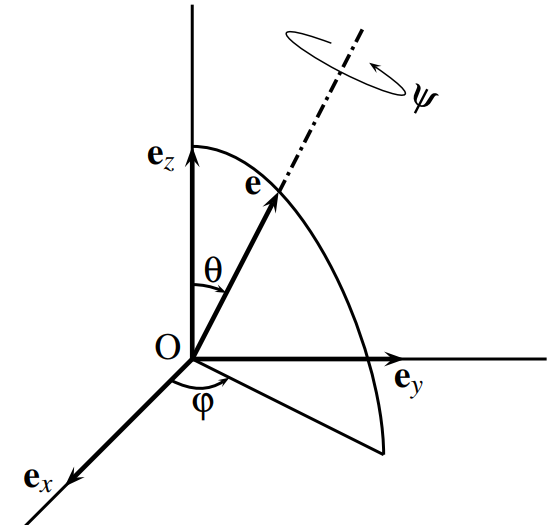
\includegraphics[width=7cm]{images/AnglesEuler.PNG} \end{center}
\end{tabular}










\section{Force Conservative}





\subsection{Définition}





Une force F est dite conservative si elle dérive d’un potentiel, i.e. si elle peut s’exprimer sous la forme : 
\[ \textbf{F} = - \nabla V(\textbf{s}) \]
où \emph{V} est une fonction de la position uniquement. \\
Le travail d’une force conservative déplaçant sont point d’application entre deux points A et B ne dépend pas du chemin \emph{C} suivi pour aller de A à B, i.e.
\[ \int_C \textbf{F} \cdot d \textbf{s} = - \int_C \nabla V \cdot d \textbf{s} = V(\textbf{s}_A) - V(\textbf{s}_B) \]





\subsection{Puissance}





Une force \textbf{F} est dite conservative si elle dérive d’un potentiel, i.e. si elle peut s’exprimer sous la forme : 
\[ \textbf{F} = − \nabla V(\textbf{s}) \]
où \emph{V} est une fonction de la position uniquement. \\
Adoptant un repère cartésien de vecteurs unitaires $ \textbf{e}_x, \textbf{e}_y, \textbf{e}_z $, la puissance développée par une telle force est donnée par : 
\[ \begin{aligned}
\mathpzc{P} = \textbf{F} \cdot \dot{\textbf{s}} &= - \Big( \frac{\partial V}{\partial x} \textbf{e}_x + \frac{\partial V}{\partial y} \textbf{e}_y + \frac{\partial V}{\partial z} \textbf{e}_z \Big) \cdot (\dot{x} \textbf{e}_x + \dot{y} \textbf{e}_y + \dot{z} \textbf{e}_z) \\
&= \bigg[ \frac{\partial V}{\partial x} \frac{d x}{d t} + \frac{\partial V}{\partial y} \frac{d y}{d t} + \frac{\partial V}{\partial z} \frac{d z}{d t} \bigg] \\
&= - \frac{d V}{d t}
\end{aligned} \]









\section{Grandeurs Résultantes du Solide}






\subsection{Moment Cinétique}





\begin{tikzpicture}

\node[anchor=north west]{\textbf{Définition}: $\displaystyle \textbf{H}_O = \int \textbf{s} \wedge \dot{\textbf{s}} \; d m $};

\node[anchor=north west] at (8,0) {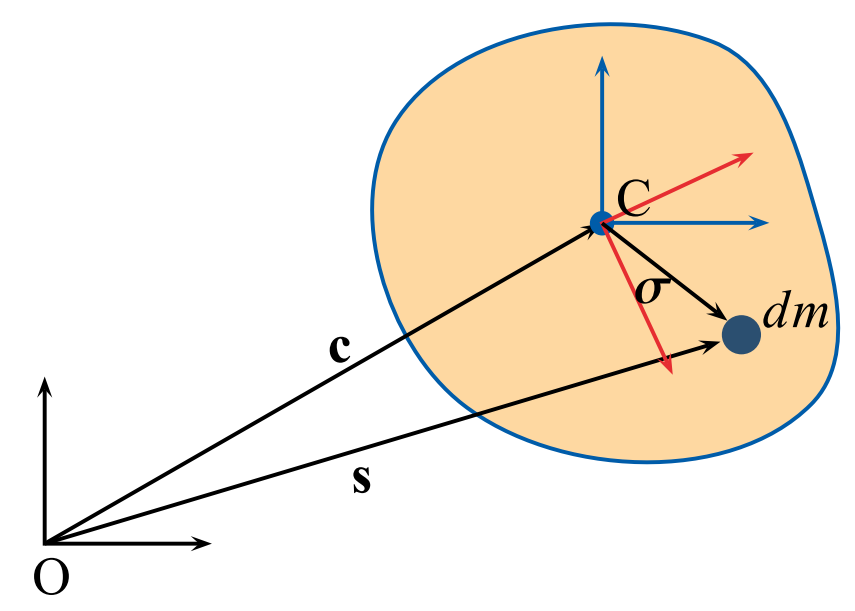
\includegraphics[width=0.4\textwidth]{images/Solide.PNG}};

\node[anchor=north west] at (0,-1) 
{$\displaystyle \textbf{H}_C = \int \boldsymbol{\sigma} \wedge \dot{\boldsymbol{\sigma}} \; d m = \int \boldsymbol{\sigma} \wedge (\boldsymbol{\omega} \wedge \boldsymbol{\sigma}) \; d m $};
\node[anchor=north west] at (0,-2) {En fait, $\displaystyle \dot{\boldsymbol{\sigma}} = \frac{\delta \boldsymbol{\sigma}}{\delta t} + (\boldsymbol{\omega} \wedge \boldsymbol{\sigma}) $ mais $\displaystyle \frac{\delta \boldsymbol{\sigma}}{\delta t} = 0 $ dans les axes liés au solide};
\node[anchor=north west] at (0,-3) {Et puisque, $ \textbf{a} \wedge (\textbf{b} \wedge \textbf{c}) = \textbf{b} (\textbf{a} \cdot \textbf{c}) - \textbf{c} (\textbf{a} \cdot \textbf{b}) $, on a:};
\draw[-] (-0.1,-2) -- (0.5,-2); \draw[-] (-0.1,-4) -- (0.5,-4); \draw[-] (-0.1,-2) -- (-0.1,-4);
\node[anchor=north west] at (0,-4)
{$ \begin{aligned}
\displaystyle \textbf{H}_C &= \int \boldsymbol{\sigma} \wedge (\boldsymbol{\omega} \wedge \boldsymbol{\sigma}) \; d m = \int \boldsymbol{\omega} \; \sigma^2 - \boldsymbol{\sigma} \; (\boldsymbol{\sigma} \cdot \boldsymbol{\omega}) \; d m \\
&= \int \boldsymbol{\omega} \cdot \big( \sigma^2 \; \textbf{I} - \boldsymbol{\sigma} \; \boldsymbol{\sigma} \big) \; d m
\end{aligned} $};

\end{tikzpicture}

Le tenseur d'inertie du solide en C étant donné par : $\displaystyle \textbf{J}_C = \int \big( \sigma^2 \; \textbf{I} - \boldsymbol{\sigma} \; \boldsymbol{\sigma} \big) \; d m $, le moment cinétique s'écrit: 
\[ \textbf{H}_C = \boldsymbol{\omega} \cdot \textbf{J}_C \]





\subsection{Énergie cinétique}





\textbf{Définition}: $\displaystyle T_O = \frac{1}{2} \int \dot{\textbf{s}} \cdot \dot{\textbf{s}} \; d m $
\[ \begin{aligned}
T_C &= \frac{1}{2} \int \big( \boldsymbol{\omega} \wedge \boldsymbol{\sigma} \big) \cdot \big( \boldsymbol{\omega} \wedge \boldsymbol{\sigma} \big) \; d m  \qquad \qquad \big[ \textbf{a} \cdot (\textbf{b} \wedge \textbf{c}) = \textbf{b} \cdot (\textbf{c} \wedge \textbf{a}) \big] \\
&= \frac{1}{2} \int \boldsymbol{\omega} \big[ \boldsymbol{\sigma} \wedge \cdot (\boldsymbol{\omega} \wedge \boldsymbol{\sigma}) \big] \; d m \\
&= \frac{1}{2} \boldsymbol{\omega} \cdot \textbf{H}_C = \frac{1}{2} \boldsymbol{\omega} \cdot \textbf{J}_C \cdot \boldsymbol{\omega}
\end{aligned} \]





\subsection{Remarque}





On a: $ \textbf{H}_C = \boldsymbol{\omega} \cdot \textbf{J}_C $, et: $ T_O = \frac{1}{2} \boldsymbol{\omega} \cdot \textbf{J}_C \cdot \boldsymbol{\omega} $, pour tout système d’axes parallèles à des axes inertiaux et centrés en un point \emph{B} fixe par rapport au solide. Le mouvement du solide par rapport à un tel référentiel se réduit à un mouvement de rotation.










\section{Équations d'Euler}





Les équations d’Euler sont les équations scalaires obtenues en projetant sur les axes principaux d’inertie d’un solide le théorème du moment cinétique rapporté à des axes centrés au centre d’inertie (ou en un point fixe du solide) et constamment parallèles à des axes inertiaux, i.e.
\[ \begin{cases}
J_1 \dot{\omega}_1 + (J_3 - J_2) \; \omega_2 \omega_3 = M_1 \\
J_2 \dot{\omega}_2 + (J_1 - J_3) \; \omega_1 \omega_3 = M_2 \\
J_3 \dot{\omega}_3 + (J_2 - J_1) \; \omega_2 \omega_1 = M_3
\end{cases} \]
où $ (\omega_1, \omega_2, \omega_3) $ et $ (M_1, M_2, M_3) $ désignent les composantes dans les axes principaux d’inertie du vecteur de Poisson et du moment des forces appliquées au solide et où $ J_1, J_2, J_3 $ sont les moments principaux d’inertie.










\section{Système à Masse Variable}





Dans quels cas, l'équation de Newton: $\displaystyle \frac{d}{d t} \big( m \dot{\textbf{s}} \big) = \textbf{F} $, permet-elle de décrire le mouvement d'un système à masse variable ? Justifier.

L’équation du mouvement d’un point matériel de masse variable soumis à une force \textbf{F} s’écrit :
\begin{equation}\tag{1}
m \frac{d \dot{\textbf{s}}}{d t} = \textbf{F} + \textbf{P} = \textbf{F} + \frac{d m}{d t} \textbf{w}
\end{equation}
puisque la poussée \textbf{P} est donnée par : $\displaystyle \textbf{P} = \frac{d m}{d t} \textbf{w} $, où \textbf{w} est la vitesse relative par rapport au système à masse variable des matières qui vont être absorbées ou qui ont été éjectées. \\
L’équation donnée : $\displaystyle \frac{d}{d t} \big( m \; \dot{\textbf{s}} \big) = \textbf{F} $, peut s’écrire : 
\begin{equation}\tag{2}
m \frac{d \dot{\textbf{s}}}{d t} = \textbf{F} - \frac{d m}{d t} \dot{\textbf{s}}
\end{equation}
Les expressions (1) et (2) ne sont équivalentes que si : $ \textbf{w} = − \dot{\textbf{s}} $, c’est-à-dire si les matières qui vont être absorbées ou qui ont été éjectées sont au repos absolu.










\section{Bifurcation}





\begin{center} \begin{tikzpicture}

\draw[->] (7,0) -- (9,0) node[right] {$ n $};
\draw[->] (0,-3.5) -- (0,3.5) node[right] {$ \theta $};
\draw[-, line width=2] node[left] {$ 0 $} (0,0) -- node[anchor=south]{stable} (3,0);
\draw[-, dashed] (3,0) -- node[anchor=south]{instable} (7,0);

\draw[color=black, smooth, line width=2, domain=3:6]   plot (\x,{ - 1.5 * sqrt(\x - 3) }) node[right]{stable};
\draw[color=black, smooth, line width=2, domain=3:6]   plot (\x,{ + 1.5 * sqrt(\x - 3) }) node[right]{stable};

\node [xshift = 2cm, yshift = -1cm] {$ n^* $};
\draw[->] (2.2,-0.8) -- (2.9,-0.1);

\end{tikzpicture} \end{center}

Ici, on a représenté les positions d'équilibre (stables et instables) de $ \theta $, qui est le seul degré de liberté du système, en fonction du paramètre \emph{n}. Pour une valeur $ n = n^* $, l'origine cesse d'être une position d'équilibre stable. Elle devient instable. En même temps, deux positions d'équilibre stable symétrique par rapport à l'origine apparaissent. \\
Ce phénomène constitue une bifurcation que l'on qualifie généralement de bifurcation surcritique.










\section{Orbite Géostationnaire}





L’orbite géostationnaire est l’orbite équatoriale pour laquelle la vitesse angulaire de rotation du satellite autour de la Terre est précisément égale à la vitesse de rotation de la Terre sur elle-même. Tous les satellites de communication sont placés en orbite géostationnaire afin de rester à l’aplomb de la zone qu’ils doivent desservir. \\
Le rayon de l’orbite géostationnaire GEO est donné par :
\[ R_{\text{GEO}} = \sqrt[3]{\frac{G M T^2}{4 \pi^2}} \]
où \emph{T} est égal à un jour sidéral, \emph{M} est la masse de la Terre et \emph{G} la constante de Cavendish. L’altitude d’une telle orbite est approximativement de 35 800 kilomètres.










\section{Orbite de Transfert de Hohmann}





\begin{tikzpicture}

\node[anchor=north west]{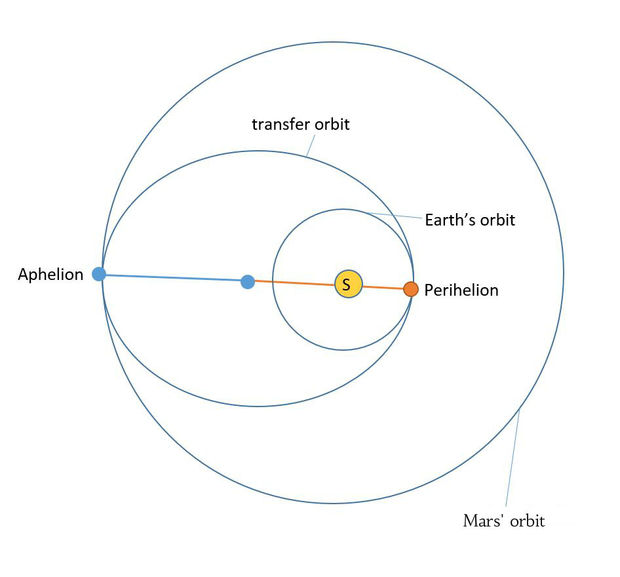
\includegraphics[width=0.5\textwidth]{images/Hohmann.jpg}};
\node[anchor=north west, text width=8cm] at (8,-2.5) {Le passage entre deux orbites circulaires coplanaires peut se faire avec une faible dépense d'énergie en suivant une orbite elliptique tangente aux deux orbites circulaires. \\ Cette orbite est appelée orbite de transfert de Hohmann.};

\end{tikzpicture}










\section{Centre de Percussion}





\begin{center}
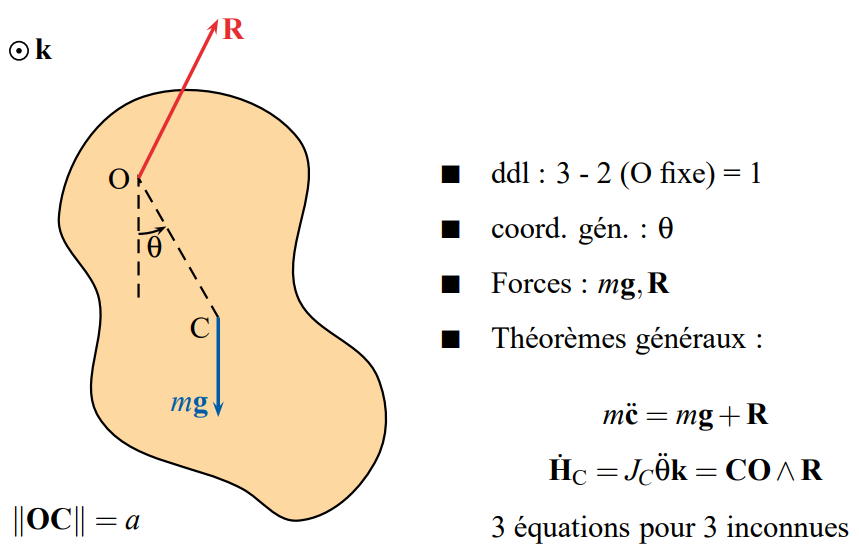
\includegraphics[width=0.49\textwidth]{images/Pendule01.PNG}
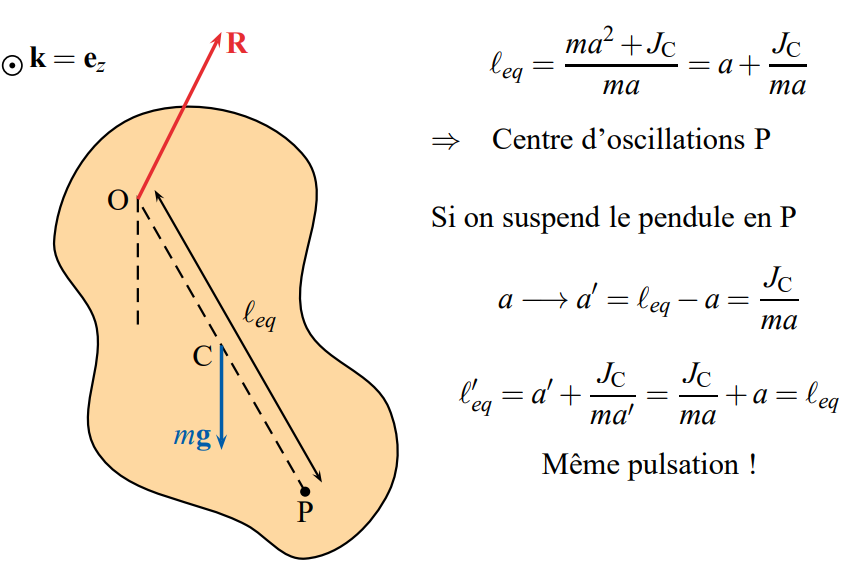
\includegraphics[width=0.49\textwidth]{images/Pendule02.PNG}
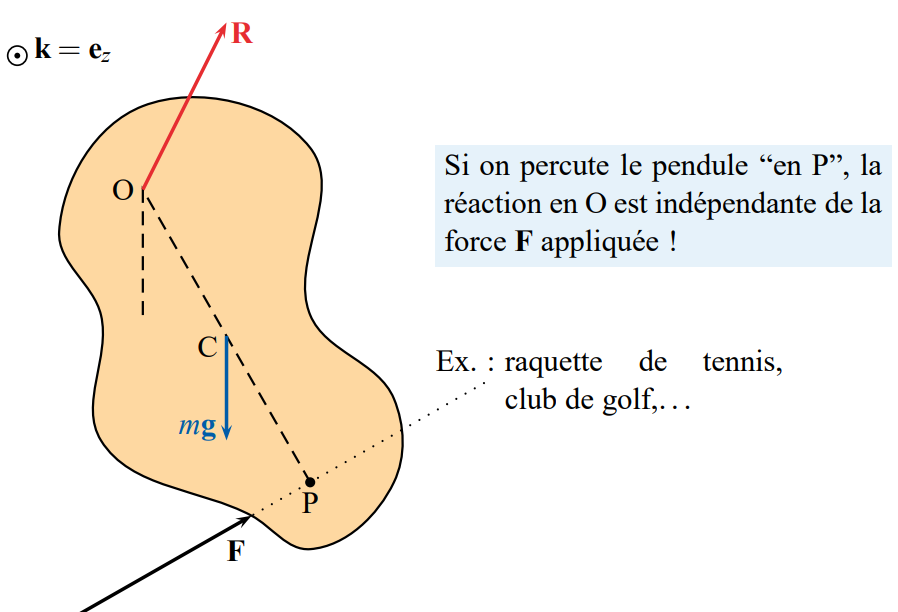
\includegraphics[width=0.49\textwidth]{images/Pendule03.PNG}
\end{center}
Le centre de percussion d’un solide est le point auquel on peut appliquer des forces extérieures arbitrairement grandes, comme les forces impulsionnelles appliquées lors d’une percussion, sans provoquer de réaction aux appuis. \\
En frappant une boule de billard de rayon \emph{R} en son centre de percussion, situé à une distance $ 2 R / 5 $ au-dessus du centre d’inertie, on communique à la boule une vitesse de translation et une vitesse de rotation compatibles avec le roulement sans glissement sans qu’aucune force de frottement ne doive être mise en oeuvre au point de contact avec le plan. \\
Dans le cas d’une raquette de tennis, le centre de percussion correspond au point du tamis où il convient de frapper la balle pour éviter de faire naître un force de réaction importante au niveau du poignet.










\section{Précession}





\subsection{Euler-Poinsot \& Précession Uniforme}





\textbf{Définition}: Le mouvement d'un solide autour d'un de ses points fixes et par rapport auquel le moment des forces extérieures est nul est appelé mouvement de Poinsot.

\textbf{Définition}: Le mouvement d'un solide autour de son centre d'inertie et soumis à des forces appliquées uniquement en ce point (comme \textbf{G}) est appelé mouvement d'Euler-Poinsot.
\begin{center}
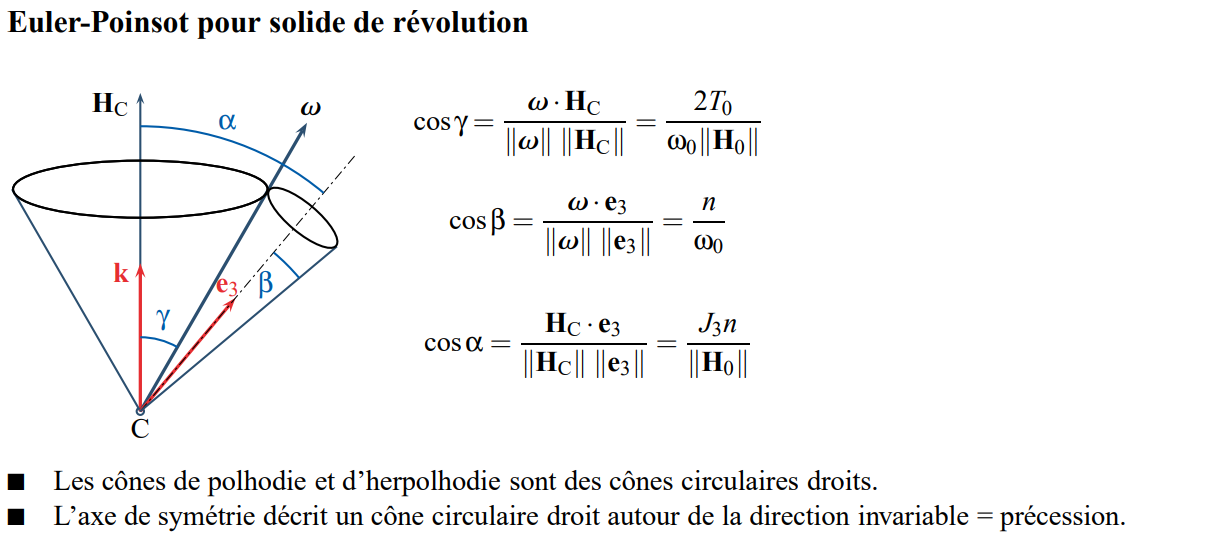
\includegraphics[width=0.8\textwidth]{images/Precession01.PNG}
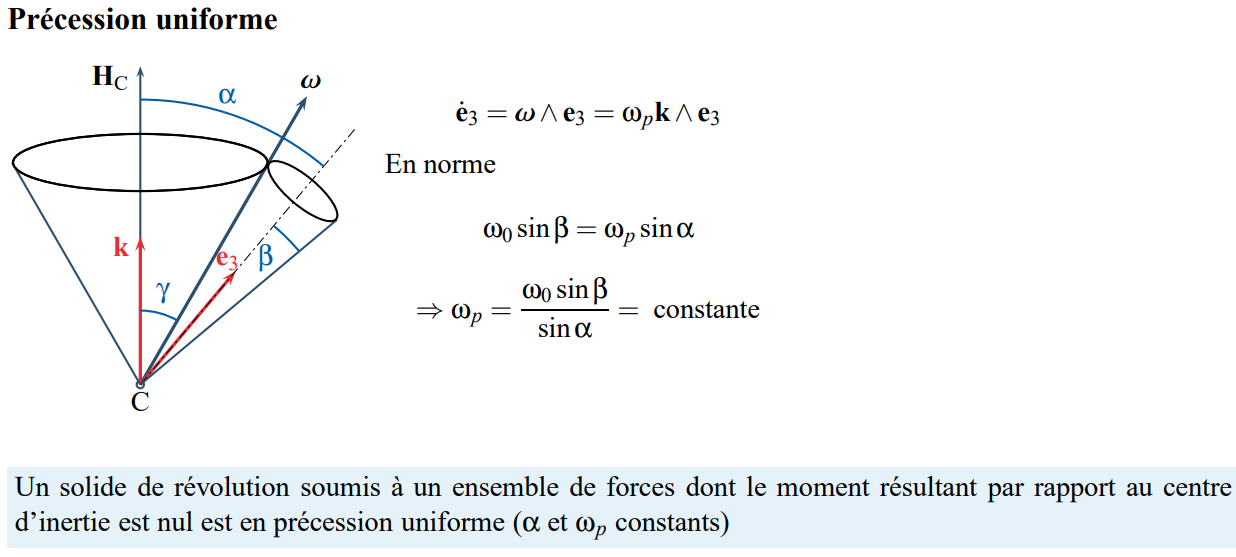
\includegraphics[width=0.8\textwidth]{images/Precession02.PNG}
\end{center}
Remarque: le cône d'herpolhodie est le cône central, celui de polhodie étant le petit à coté.





\subsection{Précession/Effet Gyroscopique}





La précession gyroscopique ou effet gyroscopique est le mouvement de précession que présente un solide de révolution en rotation rapide autour de son axe de symétrie lorsqu’il est sollicité par un couple extérieur \textbf{C} indépendant de la vitesse de rotation. Au lieu de basculer dans la direction du couple appliqué, le solide acquiert un mouvement de rotation qui tend à aligner son axe de symétrie avec la direction du couple appliqué. Au premier ordre, la vitesse de précession : $ \dot{\upvarphi} \textbf{e}_z $, est telle que : 
\[ \textbf{C} = \Gamma \dot{\upvarphi} \; \textbf{e}_z \wedge \dot{\Uppsi} \; \textbf{e} \]
où $ \Gamma $ désigne le moment d’inertie du solide par rapport à son axe de symétrie de révolution, \textbf{e} est le vecteur unitaire porté par cet axe de symétrie et : $ \dot{\Uppsi} >> \dot{\upvarphi} $, est la vitesse de rotation autour de cet axe.





\subsection{Précession Uniforme d'un Gyroscope}





On dit d’un gyroscope qu’il présente un mouvement de précession uniforme lorsque son axe de symétrie conserve une inclinaison constante par rapport à une direction fixe et tourne à vitesse angulaire constante autour de celle-ci. Dans ce mouvement, on a :
\[ \theta = \text{constante,} \qquad \dot{\upvarphi} = \text{constante,} \qquad \dot{\Uppsi} = \text{constante} \]

\begin{siderules}
Établissez l’expression du couple extérieur à appliquer à un gyroscope pour produire un mouvement de précession uniforme autour de son centre d’inertie.
\end{siderules}

 Lorsqu'on a un mouvement de précession uniforme, on a : $\displaystyle \boldsymbol{\omega} = \dot{\upvarphi} \; \textbf{e}_z + \dot{\Uppsi} \; \textbf{e} $, où $ \dot{\upvarphi} $ et $ \dot{\Uppsi} $ sont constantes. \\
Le gyroscope possède un tenseur central d'inertie de la forme : $\displaystyle \textbf{J}_C = A \; \textbf{I} + (\Gamma - A) \; \textbf{e} \textbf{e} $, où $ \Gamma $ et \emph{A} sont, respectivement, les moments principaux d’inertie pour la rotation autour de \textbf{e} et autour de tout axe perpendiculaire à \textbf{e}. \\
On calcule dès lors, 
\[ \textbf{H}_C = \textbf{J}_C \cdot \boldsymbol{\omega} = A \; \boldsymbol{\omega} + (\Gamma - A) \; (\dot{\Uppsi} + \dot{\upvarphi} \cos \theta) \; \textbf{e} \]
\[ \begin{aligned}
\dot{\textbf{H}}_C &= A \; \dot{\boldsymbol{\omega}} + (\Gamma - A) \; (\dot{\Uppsi} + \dot{\upvarphi} \cos \theta) \; \dot{\textbf{e}} \\
&= \dot{\upvarphi} \; \big[ \Gamma \dot{\Uppsi} + (\Gamma - A) \; \dot{\upvarphi} \cos \theta \big] \; \textbf{e}_z \wedge \textbf{e}
\end{aligned} \]
Appliquant le théorème du moment cinétique en \emph{C}, on en déduit que, pour provoquer une précession uniforme, il convient d’appliquer un couple extérieur de moment : 
\[ \textbf{M}_C = \dot{\upvarphi} \; \big[ \Gamma \dot{\upvarphi} + (\Gamma - A) \; \dot{\upvarphi} \cos \theta \big] \; \textbf{e}_z \wedge \textbf{e} \]
à la fois perpendiculaire à l’axe de symétrie du gyroscope et à l’axe autour duquel il précesse.






\subsection{Supplément}





\textbf{Définition de la stabilisation - rigidité gyroscopique}: un solide présentant une très grande vitesse de rotation autour d’un axe de symétrie ‘résiste’ aux sollicitations extérieures.

\begin{center}
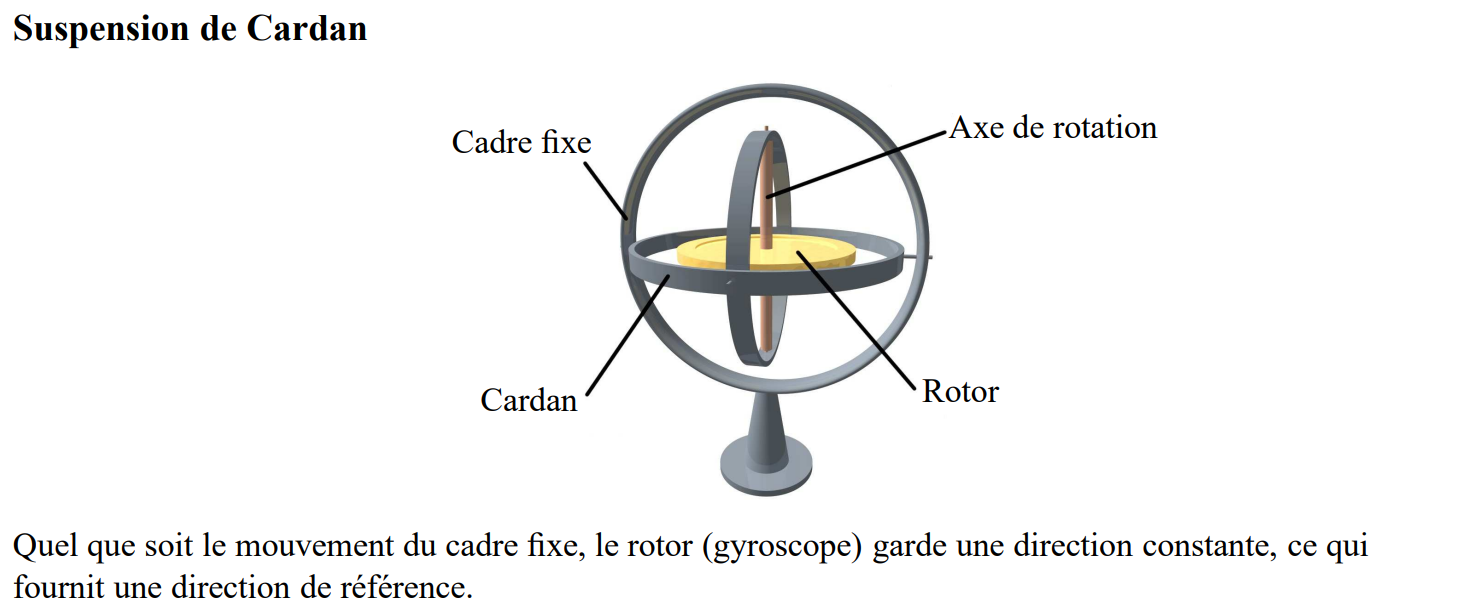
\includegraphics[width=0.8\textwidth]{images/Cardan.PNG}
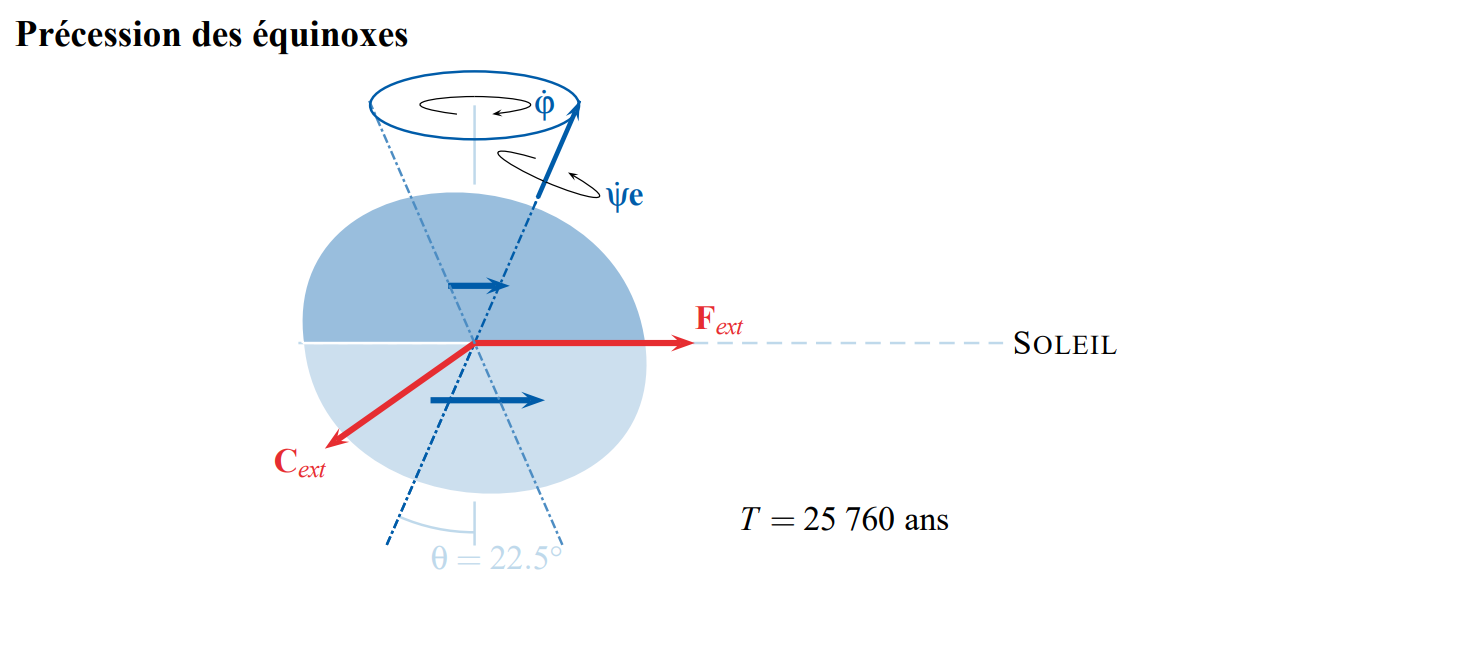
\includegraphics[width=0.8\textwidth]{images/Precession03.PNG}
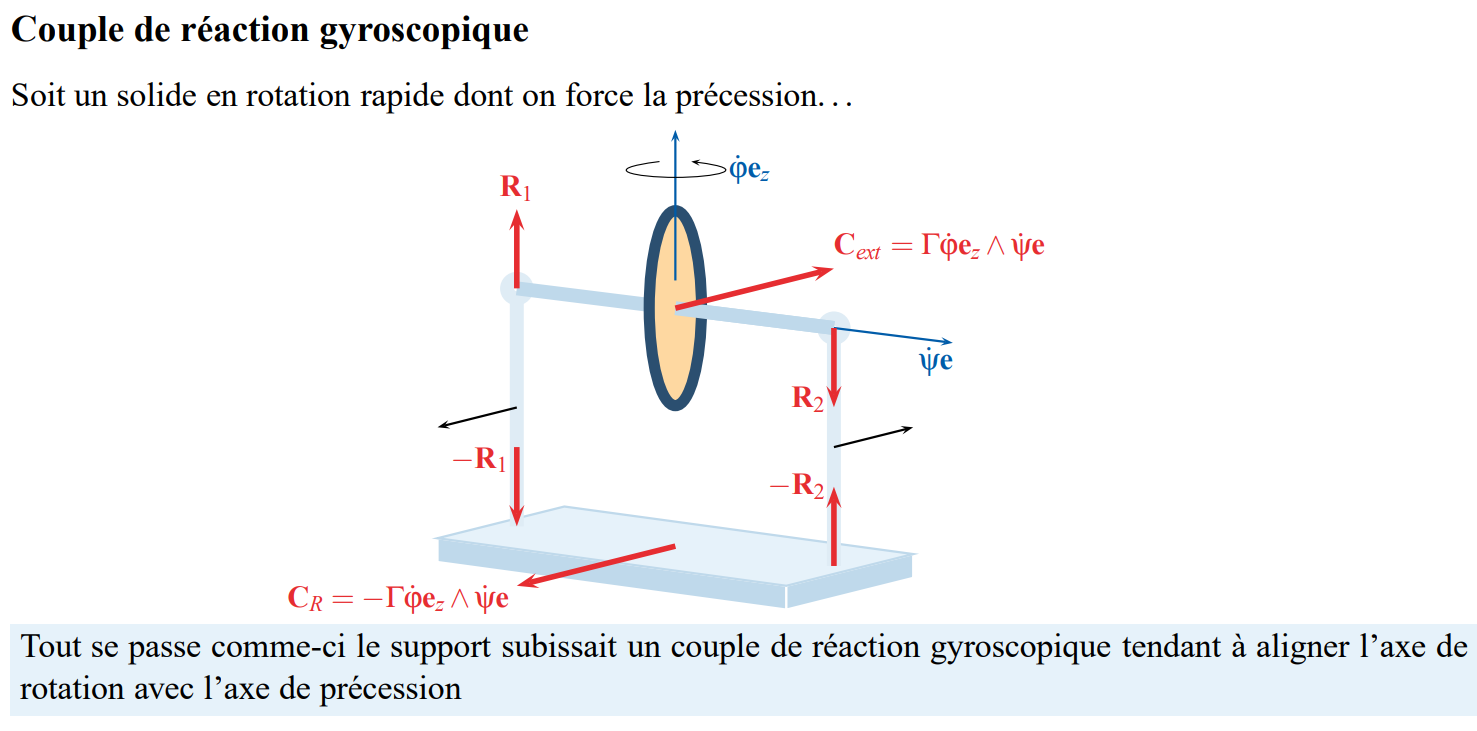
\includegraphics[width=0.8\textwidth]{images/Precession04.PNG}
\end{center}









\section{Toupie}





On considère une toupie présentant une symétrie de révolution d’axe \textbf{e} en mouvement autour de son sommet O fixe.





\subsection{Tenseur d'Inertie}





Le tenseur d'inertie s'écrit : $ \textbf{J}_O = J_1 \; \textbf{e}_1 \textbf{e}_1 + J_2 \; \textbf{e}_2 \textbf{e}_2 + \Gamma \; \textbf{e} \textbf{e} $, où $ \textbf{e}_1 $ et $ \textbf{e}_2 $ sont deux axes perpendiculaires à \textbf{e}. \\
Vu la symétrie de révolution, le solide présente le même moment d’inertie pour la rotation autour de tout axe perpendiculaire à \textbf{e} et passant par le point O. Dès lors, $ J_1 = J_2 = A $ et : 
\[ \textbf{J}_O = A \; \textbf{e}_1 \textbf{e}_1 + A \; \textbf{e}_2 \textbf{e}_2 + \Gamma \; \textbf{e} \textbf{e} = A \; \textbf{I} + (\Gamma - A) \; \textbf{e} \textbf{e} \]





\subsection{Moment Cinétique}





Puisque la toupie est en rotation autour de son sommet O fixe, on a : $ \textbf{H}_O = \textbf{J}_O \cdot \boldsymbol{\omega} $. Les forces appliquées à la toupie sont :

\begin{tabular}{M{7cm}M{8cm}}
\begin{itemize}
    \item la force de pesanteur, assimilable à une force unique $ m \textbf{g} $ appliquée au centre d’inertie de la toupie ;
    \item la réaction \textbf{R} appliquée au point O.
\end{itemize}
Dès lors, le théorème du moment cinétique s’écrit : 
\[ \dot{\textbf{H}}_O = \textbf{M}_O = h \; \textbf{e} \wedge (m \textbf{g}) = - m g h \; \textbf{e} \wedge \textbf{e}_z \]
&
\begin{center} 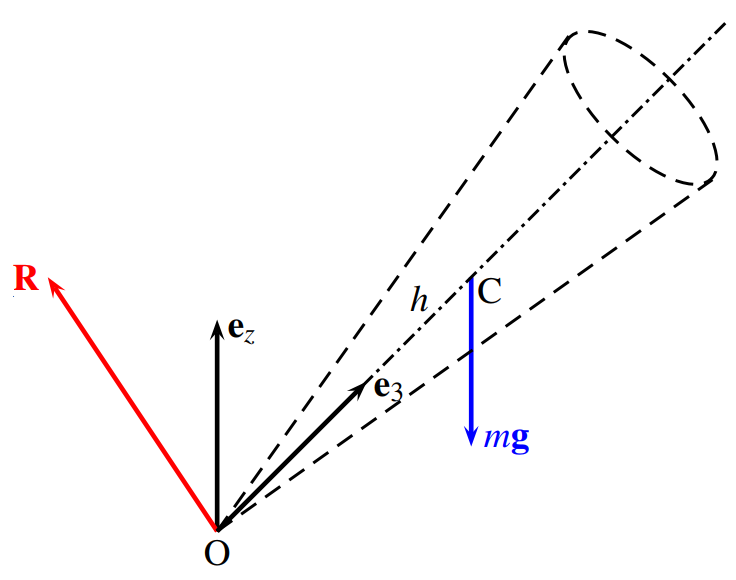
\includegraphics[width=7cm]{images/Toupie01.PNG} \end{center}
\end{tabular}





\subsection{Intégrales Premières}





On peut obtenir 3 intégrales premières: 
\begin{enumerate}

\item $ T_O + V_{m g} = E $, qui exprime la conservation d'énergie du système.
\item $ \textbf{H}_O \cdot \textbf{e}_z = H_z $, qui exprime la conservation de la composante verticale du moment cinétique.
\item $ \textbf{e} \cdot \textbf{H}_O = \Gamma \; \textbf{e} \cdot \boldsymbol{\omega} = \text{const.} $, cette intégrale première exprime la conservation du \emph{spin} : $ n = \textbf{e} \cdot \boldsymbol{\omega} $.

\end{enumerate}

\textbf{Démonstration de la n°3}: \\
En projetant sur \textbf{e}, il vient : $ \textbf{e}_z \cdot \dot{\textbf{H}}_O = 0 $. On utilise la dérivée relative par rapport aux axes liés au solide et l'équation devient :
\[ \textbf{e} \cdot \bigg[ \frac{\delta \textbf{H}_O}{\delta t} + \boldsymbol{\omega} \wedge \textbf{H}_O \bigg] = 0 \]
où : $\displaystyle \textbf{H}_O = \textbf{J}_O \cdot \boldsymbol{\omega} = A \boldsymbol{\omega} + (\Gamma - A) \; (\textbf{e} \cdot \boldsymbol{\omega}) \; \textbf{e} $ \\
$\displaystyle \implies \boldsymbol{\omega} \wedge \textbf{H}_O = (\Gamma - A) \; (\textbf{e} \cdot \boldsymbol{\omega}) \; (\boldsymbol{\omega} \wedge \textbf{e}) $ \\
$\displaystyle \implies \textbf{e} \cdot (\boldsymbol{\omega} \wedge \textbf{H}_O) = 0 $ \\
de sorte que, puisque \textbf{e} est constant dans les axes liés à la toupie, $\displaystyle \textbf{e} \cdot \frac{\delta \textbf{H}_O}{\delta t} = \frac{\delta}{\delta t} \big( \textbf{e} \cdot \textbf{H}_O \big) = 0 $. \\
Dès lors,
\[ \textbf{e} \cdot \textbf{H}_O = \Gamma \; \textbf{e} \cdot \boldsymbol{\omega} = \text{const.} \]





\subsection{Énergie Cinétique}





La toupie étant en rotation autour de son sommet O fixe, son énergie cinétique peut être exprimée avec les angles d'Euler sous la forme :
\[ \begin{aligned}
T_O &= \frac{1}{2} \boldsymbol{\omega} \cdot \textbf{J}_C \cdot \boldsymbol{\omega} = \frac{1}{2} \boldsymbol{\omega} \cdot \big[ A \; \textbf{I} + (\Gamma - A) \; \textbf{e} \textbf{e} \big] \cdot \boldsymbol{\omega} \\
&= \frac{A}{2} \omega^2 + \frac{1}{2} (\Gamma - A) \; (\boldsymbol{\omega} \cdot \textbf{e})^2 \\
&= \frac{A}{2} \big( \dot{\upvarphi}^2 + \dot{\Uppsi}^2 + \dot{\theta}^2 + \dot{\Uppsi} \dot{\upvarphi} \cos \theta \big) + \frac{1}{2} (\Gamma - A) \; (\dot{\Uppsi} + \dot{\upvarphi} \cos \theta)^2
\end{aligned} \]










\section{Types de Mouvement d'une Toupie}





\begin{enumerate}

    \item Précession monotone.
    \item Précession de signe variable.
    \item Mouvement avec rebroussement.
    \item Précession uniforme.
    \item Mouvement asymptotique.
    \item Toupie forte.

\end{enumerate}

\begin{center}
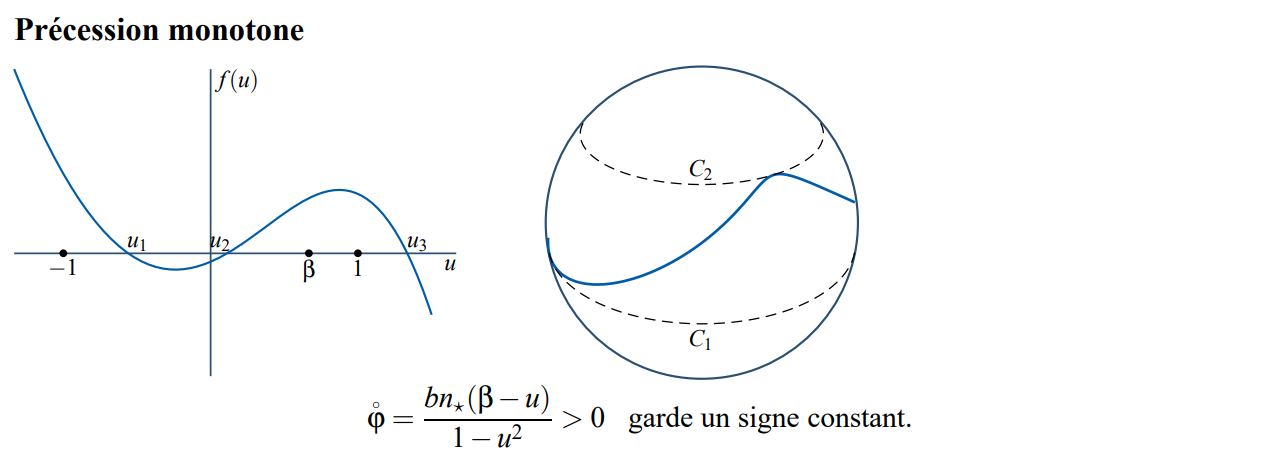
\includegraphics[width=0.8\textwidth]{images/Toupie02.PNG}
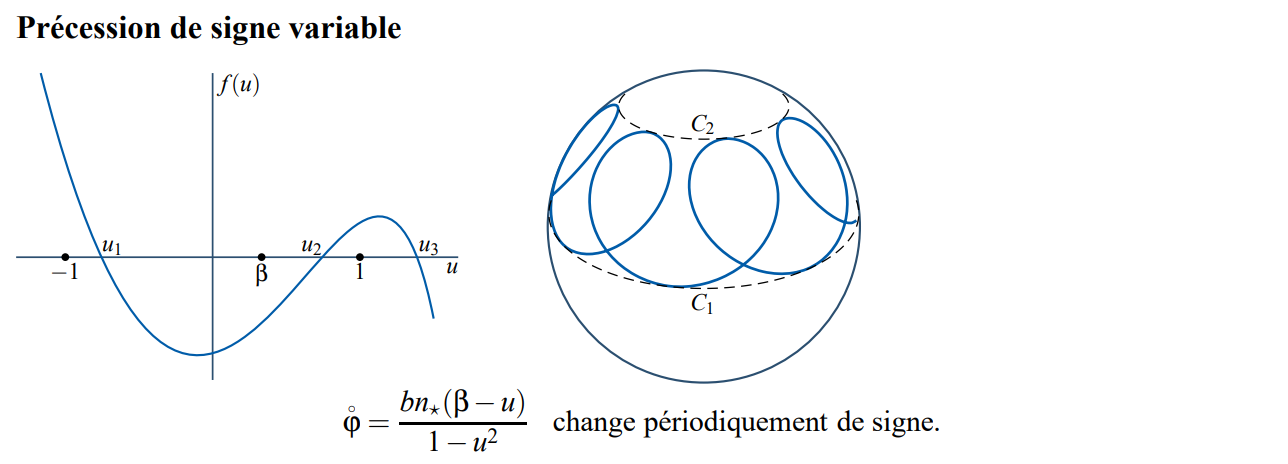
\includegraphics[width=0.8\textwidth]{images/Toupie03.PNG}
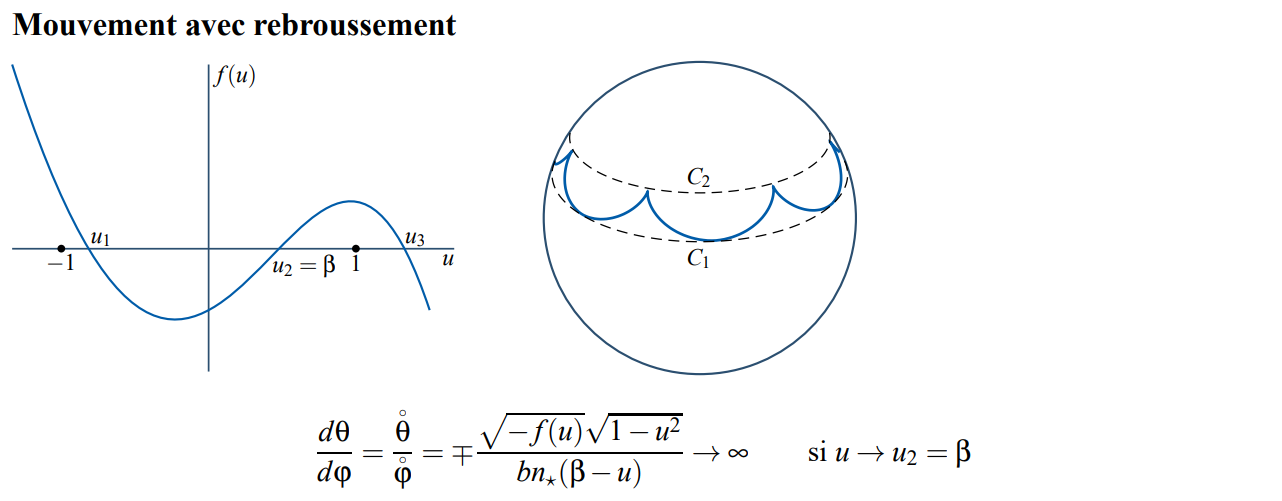
\includegraphics[width=0.8\textwidth]{images/Toupie04.PNG}
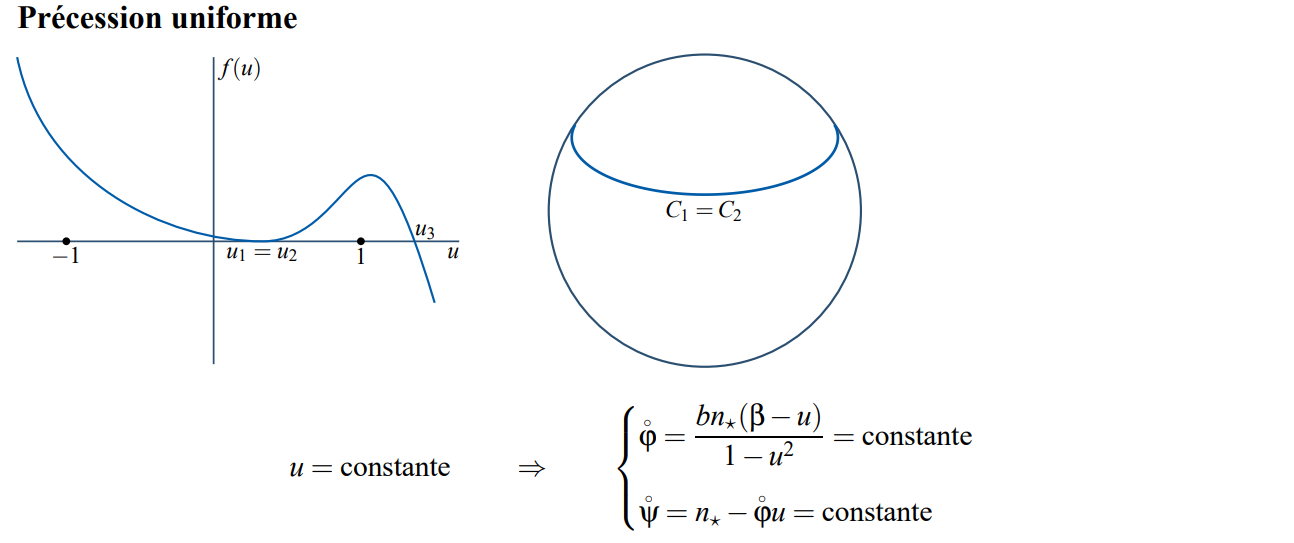
\includegraphics[width=0.8\textwidth]{images/Toupie05.PNG}
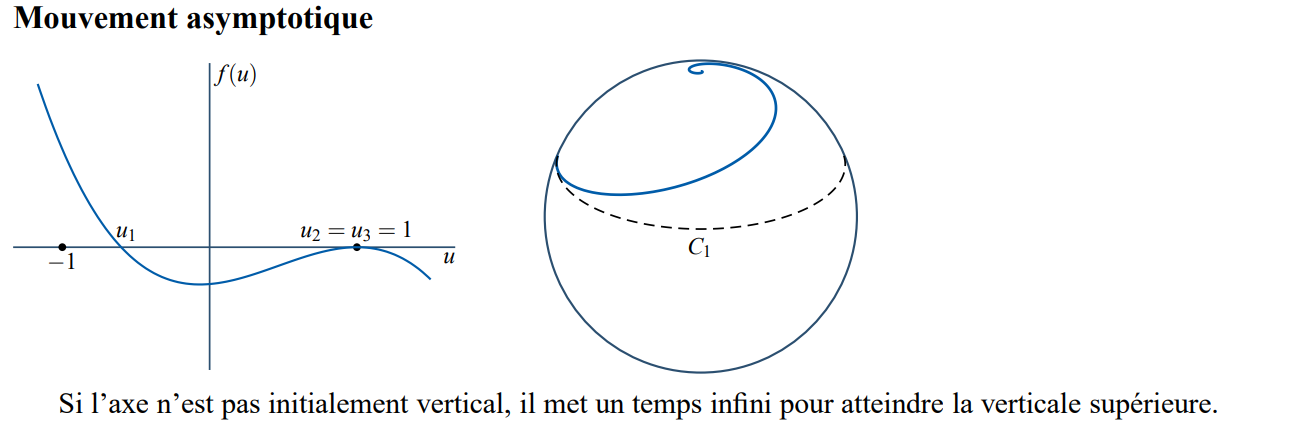
\includegraphics[width=0.8\textwidth]{images/Toupie06.PNG}
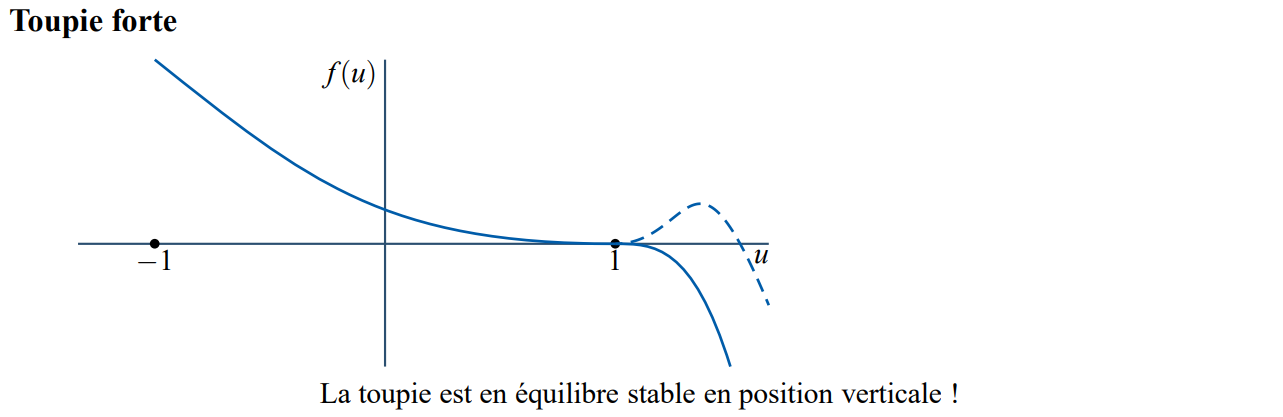
\includegraphics[width=0.8\textwidth]{images/Toupie07.PNG}
\end{center}





\subsection{Précession Uniforme}





Le mouvement de précession uniforme d’une toupie est un mouvement caractérisé par l’absence de nutation et par des vitesses de précession et de rotation propre constantes. L’axe de la toupie garde donc une inclinaison constante par rapport à la verticale autour de laquelle il tourne à vitesse angulaire constante. La toupie tourne aussi sur elle-même à vitesse constante.






\subsection{Toupie Forte}





La toupie forte est un solide de révolution dont la rotation rapide autour de son axe de symétrie de révolution assure l’équilibre stable dans la position verticale supérieure. La toupie reste verticale en dépit de la force de pesanteur qui tend à faire basculer son axe de rotation lors de toute perturbation de l’équilibre.










\section{Équilibrage Statique et Dynamique d’un Système Tournant}





L’équilibrage statique d’un système tournant consiste à veiller à ce que le centre d’inertie du système soit situé sur l’axe de rotation.  \\
L’équilibrage dynamique, quant à lui, consiste à veiller à ce que l’axe de rotation \textbf{e} corresponde à un axe principal d’inertie du système.

Pour réaliser l’équilibrage statique et dynamique, on peut ajouter de petits balourds sur le système (ou enlever de la matière en effectuant quelques perforations). Pour un système en rotation autour d’un axe fixe unique, deux balourds sont suffisants pour réaliser cette opération. \\
Si un système non équilibré est mis en rotation, des réactions parasites sont induites au niveau des appuis, lesquelles engendrent des sollicitations mécaniques parasites qui peuvent endommager le système ou son support.










\section{Forces de Cohésion/Internes}





Les forces intérieures agissant au sein d'un solide rigide sont notées \textbf{f}, ainsi $ \textbf{f}_{ji} $ est la force qu'un point \emph{j} exerce sur un point \emph{i} du même système.

Au vu du principe de l'action et de la réaction, il est évidemment intéressant de regrouper deux à deux les forces intérieures qui se correspondent. En effet, on a:
\[ \textbf{f}_{ij} = - \textbf{f}_{ji} \]
La résultante de ces forces est donc nulle. De même, on a:
\[ \textbf{s}_i \wedge \textbf{f}_{ji} + \textbf{s}_j \wedge \textbf{f}_{ij} = \textbf{0} \]
Ce qui fait que le moment résultant est nul, lui aussi. De même pour la puissance: 
\[ \dot{\textbf{s}}_i \cdot \textbf{f}_{ji} + \dot{\textbf{s}}_j \cdot \textbf{f}_{ij} = 0 \]










\section{Résultats du Théorème C pour un Système de Points}





Un système de points possède une masse: $ m = \sum m_i $, et son centre d'inertie est donné par: $ m \textbf{c} = \sum m_i \textbf{s}_i $. Les grandeurs résultantes sont facilement retrouvable, par exemple le moment cinétique est donné par: $ \textbf{H}_O = \sum m_i \textbf{s}_i \wedge \dot{\textbf{s}}_i $. Et si on veut décomposer le mouvement, on applique la méthode générale qui suit.

\begin{center}
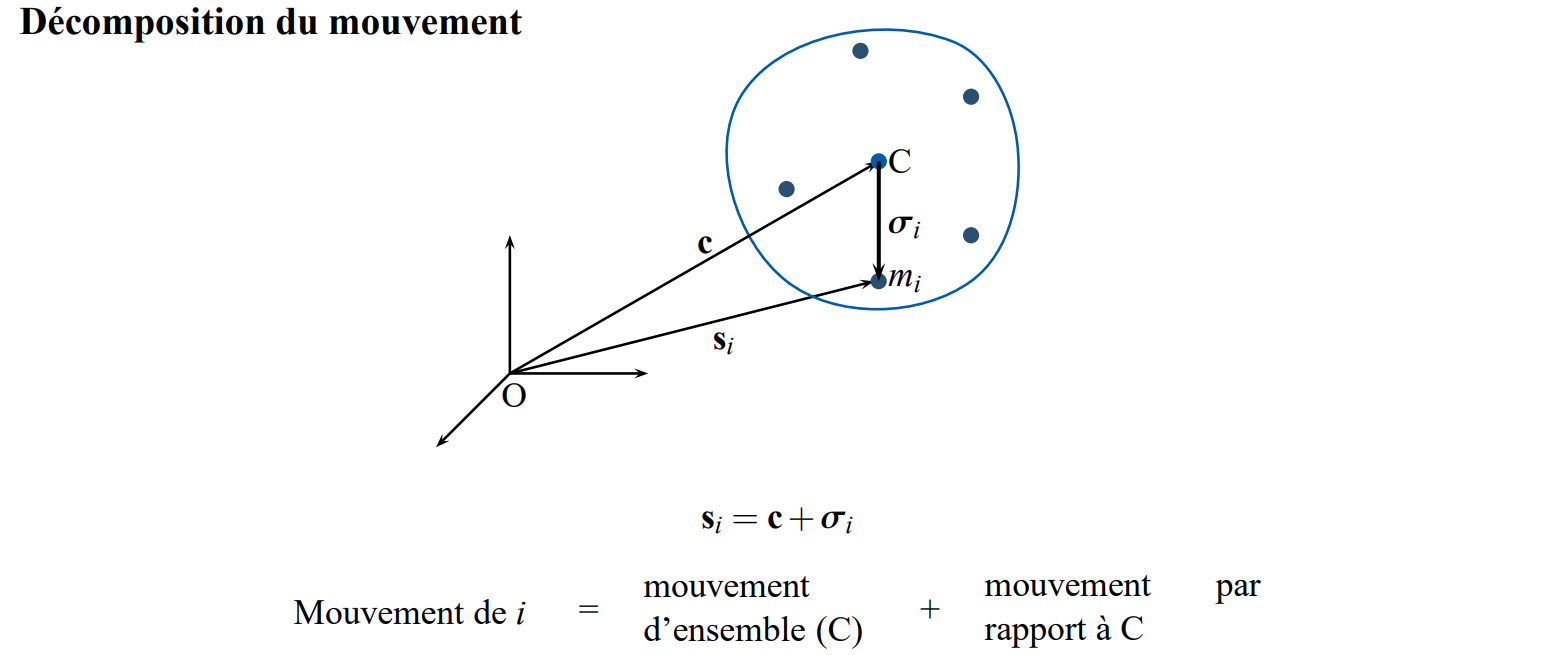
\includegraphics[width=0.8\textwidth]{images/ThC01.PNG}
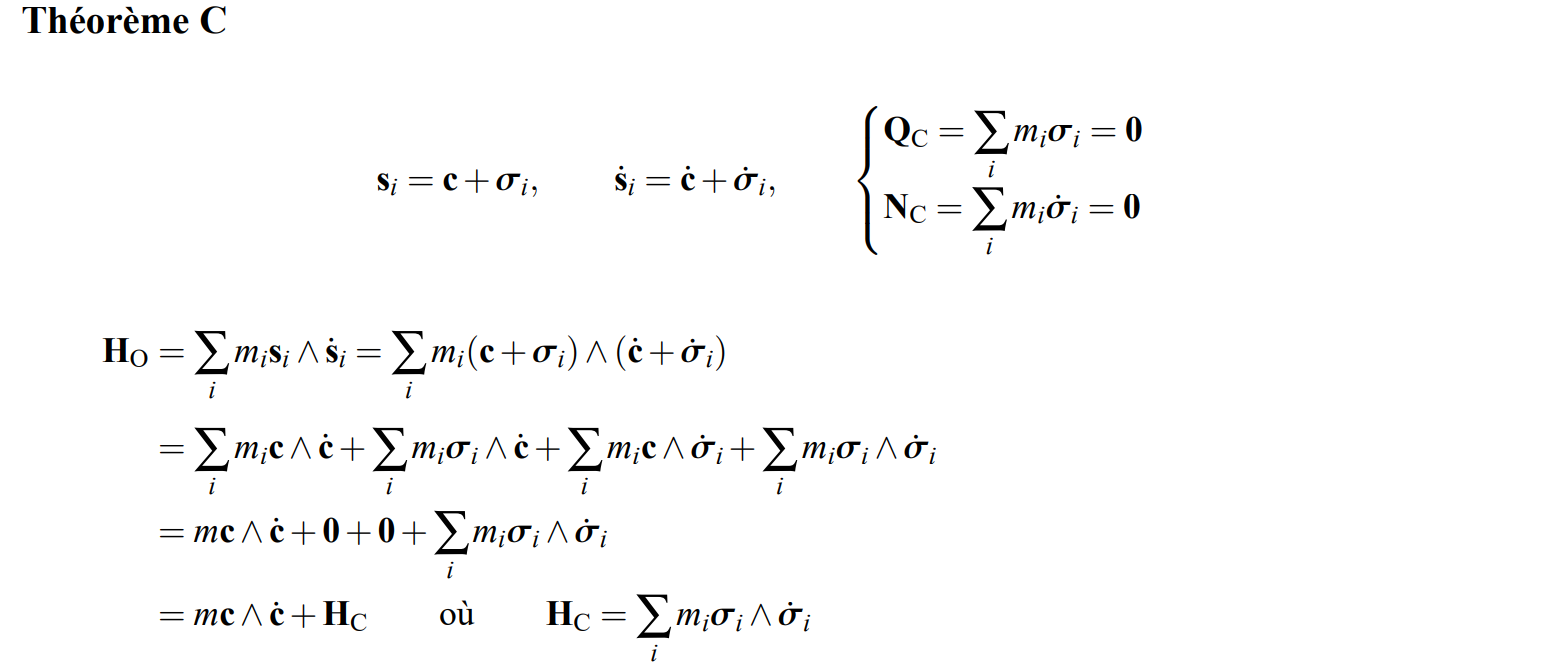
\includegraphics[width=0.8\textwidth]{images/ThC02.PNG}
\end{center}

Remarque: le moment statique $ \textbf{Q}_O $ et le moment cinétique $ \textbf{N}_O $ ne dépendent que de \textbf{c}, ce qui fait que: $ \textbf{Q}_C = \textbf{N}_C = 0 $.










\section{Axes et Moments Principaux d’Inertie d’un Solide}





Les axes principaux d’inertie en un point B sont ceux dans lesquels le tenseur d’inertie $ \textbf{J}_B $ est représenté par une matrice diagonale. Les éléments de cette matrice, i.e. les moments d’inertie pour la rotation autour des axes principaux d’inertie, sont les moments principaux d’inertie.

Les axes principaux d’inertie coïncident avec les éléments de symétrie matérielle du solide.























\newpage





















\part{Question II - Point Matériel}





On va sûrement avoir un mouvement avec une force centrale. Ça peut être un mouvement guidé mais pas forcément. On va donc appliquer la démarche suivante : 

\begin{tabular}{M{11cm}M{4cm}}
\begin{enumerate}
\item Méthode Générale - Point matériel.
\item Méthode Spécifique - Force Centrale \emph{Sans} Courbe de Guidage.
\item Méthode Spécifique - Force Centrale \emph{Avec} Courbe de Guidage.
\item Méthode Générale - Étude Stabilité.
\end{enumerate}
&
\begin{center} \begin{tikzpicture}
\node (1) [rouge, minimum width = 0.5cm, minimum height = 0.5cm, draw = none] {\textbf{1.}};
\node (2) [rouge, minimum width = 0.5cm, minimum height = 0.5cm, draw = none, fill = blue!30, xshift = -1cm, yshift = -1cm] {\textbf{2.}};
\node (3) [rouge, minimum width = 0.5cm, minimum height = 0.5cm, draw = none, fill = blue!30, xshift = 1cm, yshift = -1cm] {\textbf{3.}};
\node (4) [rouge, minimum width = 0.5cm, minimum height = 0.5cm, draw = none, yshift = -2cm] {\textbf{4.}};
\draw[->] (1) -- (2);
\draw[->] (1) -- (3);
\draw[->] (2) -- (4);
\draw[->] (3) -- (4);
\end{tikzpicture} \end{center}
\end{tabular}





\section{Méthode Générale - Point Matériel}





\begin{enumerate}





%% 
\item On commence tous les problèmes de mécanique rationnelle en \textcolor{red}{\textbf{lisant}} attentivement \textcolor{red}{\textbf{l'énoncé}} et en observant le dessin s'il y en a un.





%% 
\item Il faut \textcolor{red}{\textbf{décomposer le mouvement en}} plusieurs \textcolor{red}{\textbf{phases}} si il y a besoin (certains mouvements n'ont qu'une seule phase). Chaque phase correspond à une certaine période de temps et s'étend donc d'un temps $ t_1 $ à un temps $ t_2 $. Quand change-t-on de phase ? Lorsque il y a un changement dans les forces extérieures au système. \\
Exemples : 
\begin{itemize}
\item Dans un premier temps, la fusée expulse du gaz (\textbf{P}) puis arrête ($ \textbf{P} = \textbf{0} $).
\item Un train avance sur des rails ($ \textbf{R}_\nu $) puis déraille ($ \textbf{R}_\nu = \textbf{0} $).
\item Le courant électrique ne passe pas car le circuit est ouvert ($ \textbf{B} = \textbf{0} \implies \textbf{F}_B = \textbf{0} $) puis on le ferme ($ \textbf{B} \neq \textbf{0} \implies \textbf{F}_B \neq \textbf{0} $).
\end{itemize}





%% 
\item On \textcolor{red}{\textbf{liste}} toutes \textcolor{red}{\textbf{les données du problèmes}} qui n'ont "rien" à voir avec les forces et l'accélération. On va donc lister des données comme la masse, la position initiale/intermédiaire/finale, la vitesse ini/inter/fin, les informations en rapport avec le temps, la trajectoire, etc.





%% 
\item Maintenant, on va d'abord \textcolor{red}{\textbf{nommer le}} type de \textcolor{red}{\textbf{mouvement}} (mouvement guidé, chute libre, champ de force/force centrale, particule chargée dans un champ magnétique/électrique, masse variable, ...) puis \textcolor{red}{\textbf{lister}} toutes \textcolor{red}{\textbf{les forces}} selon les trois catégories suivantes : 
\begin{itemize}
\item \textcolor{blue}{\textbf{Force appliquée}} : 
    \begin{itemize}
    \item Gravité : $ \textbf{G} = m \textbf{g} $
    \item Champ de force/force centrale : $\displaystyle \textbf{F} = - \frac{\mu}{s^3} \textbf{s} = - m \mu r^{-2} \textbf{e}_r $
    \item Rappel d'un ressort $ \textbf{F} = - k (l - l_0) \textbf{e} = - k x \textbf{e} = - k \textbf{x} $
    \item Ressort de torsion d'axe $ \textbf{C} = - k (\theta - \theta_0) \textbf{e} = - k \theta \textbf{e} $
    \item Lorentz/électromagnétique $ \textbf{F} = q \; (\textbf{E} + \dot{\textbf{s}} \wedge \textbf{B}) $
    \item Masse variable $\displaystyle \textbf{P} = \frac{d m}{d t} \textbf{v} $
    \end{itemize}
\item \textcolor{blue}{\textbf{Force de liaison}} : 
    \begin{itemize}
    \item Tension dans une corde : proportionnelle à son extension (comme le ressort) seulement lorsque la corde est tendue et étirée.
    \item Force normale : $ \textbf{N} = \textbf{R}_\nu $.
    \item Force binormale : $ \textbf{R}_\beta $.
    \end{itemize}
La force normale est normale à la courbe/surface et la force binormale est une force de réaction normale à la courbe et à \textbf{N}. La binormale est souvent perpendiculaire au plan dans lequel se passe le mouvement.
\item \textcolor{blue}{\textbf{Force de frottement}} : 
    \begin{itemize}
    \item Frottement fluide (loi de Stokes) : $ \textbf{F} = - c \; \dot{\textbf{s}} $
    \item Frottement sec : $\displaystyle \textbf{T} = - \mu N \frac{\dot{\textbf{s}}}{\| \dot{\textbf{s}} \|} $
    \end{itemize}
\end{itemize}
Enfin, on va \textcolor{red}{\textbf{écrire ce qui est en rapport avec l'accélération}}. On note le type d'accélération (centripète, linéaire, ...).





%%
\item Puis on écrit la \textcolor{red}{\textbf{loi de Newton}} (équation différentielle vectorielle du mouvement) : 
\[ \textbf{F} = m \; \ddot{\textbf{s}} \qquad \qquad \qquad \sum \textbf{F}_{\text{extérieures}} = m \; \ddot{\textbf{s}} \]
Si le repère n'est pas inertiel, la loi de Newton s'écrit \footnote{Voir Annexe pour une explication plus détaillée.} : 
\[ \begin{aligned} m \; \textbf{a}_r = m \frac{\delta^2 \textbf{r}}{\delta t^2} &= \textbf{G} - m \; \textbf{a}_e - m \; \textbf{a}_c \\ &= \textbf{G} - m \Big[ \frac{d^2 \textbf{b}}{d t^2} + \dot{\textbf{w}} \wedge \textbf{r} + \textbf{w} \wedge (\textbf{w} \wedge \textbf{r}) \Big] - m \Big[ 2 \textbf{w} \wedge \frac{\delta \textbf{r}}{\delta t} \Big] \end{aligned} \]





%% 
\item Il faut maintenant \textcolor{red}{\textbf{tracer le dessin}}.
\begin{enumerate}
\item Premièrement, on dessine la \textcolor{blue}{\textbf{trajectoire}} du mobile dans l'espace grâce aux données sur sa provenance, sa destination, son type de mouvement (parabolique, circulaire, rectiligne, ...), etc. Il faut aussi placer le mobile sur un point quelconque de sa trajectoire.
\item Deuxièmement, on dessine toutes les \textcolor{blue}{\textbf{forces}} quelles soient appliquées, de liaison ou de frottement. On trace aussi l'\textcolor{blue}{\textbf{accélération}}.
\item Troisièmement, on dessine la \textcolor{blue}{\textbf{vitesse}} et on marque les \textcolor{blue}{\textbf{position initiales et finales}} de la phase de mouvement que l'on étudie.
\end{enumerate}

\end{enumerate}










\section{Méthode Spécifique - Force Centrale \emph{Sans} Courbe de Guidage.}





\begin{enumerate}





%%
\item Il faut montrer que \textcolor{orange}{\textbf{le mouvement est plan}}. On a deux méthodes : 
\begin{enumerate}

\item On multiplie vectoriellement l'équation du mouvement par : $ \textbf{s} = r \; \textbf{e}_r $, ce qui donne :
\[ \textbf{s} \wedge \ddot{\textbf{s}} = \textbf{0} \implies \frac{d}{d t} (\textbf{s} \wedge \dot{\textbf{s}}) = \textbf{0} \implies \textbf{s} \wedge \dot{\textbf{s}} = \textbf{h} \]
On conclut : 
\begin{siderules}
À chaque instant, le vecteur position et le vecteur vitesse sont donc perpendiculaires à un vecteur constant \textbf{h}, ce qui indique que le mouvement a lieu dans le plan perpendiculaire à \textbf{h}.
\end{siderules}
Remarque: \textbf{h} est le moment cinétique par unité de masse.

\item On place un repère absolu : O, $ \textbf{E}_x $, $ \textbf{E}_y $, $ \textbf{E}_z $. Avec : O au centre de force, $ \textbf{E}_x $ qui pointe vers le point matériel, le vecteur vitesse est initialement compris dans le plan défini par les vecteurs $ \textbf{E}_x $ et $ \textbf{E}_y $. On multiplie scalairement l'équation vectorielle du mouvement par : $ \textbf{E}_z $, ce qui donne : 
\[ \ddot{\textbf{s}} = \textbf{0} \]
Puisque l'accélération est nulle tandis que les vecteurs position et vitesse sont compris dans le plan défini plus haut ($ \perp \textbf{E}_z $), alors le mouvement est plan.

\end{enumerate}





%%
\item Il faut maintenant déterminer \textcolor{orange}{\textbf{\emph{deux} intégrales scalaires}} et préciser leur interprétation physique. Puisque le mouvement est plan, on va utiliser les coordonnées polaires. On a : $ \textbf{s} = r \; \textbf{e}_r \; ; \; \dot{\textbf{s}} = \dot{r} \; \textbf{e}_r + r \; \dot{\theta} \; \textbf{e}_\theta \; ; $
\[ \begin{aligned}
\ddot{\textbf{s}} &= \big( \ddot{r} - r \dot{\theta}^2 \big) \; \textbf{e}_r + \big( 2 \dot{r} \dot{\theta} + r \ddot{\theta} \big) \; \textbf{e}_\theta \\
&= \big( \ddot{r} - r \dot{\theta}^2 \big) \; \textbf{e}_r + \frac{1}{r} \frac{d}{d t} \big( r^2 \dot{\theta} \big) \; \textbf{e}_\theta
\end{aligned} \]
Ensuite, on combine cette équation et l'équation du mouvement que l'on projette alors sur : $ \textbf{e}_r $ et $ \textbf{e}_\theta $ pour obtenir deux équations scalaires. On intègre ensuite les équations. \textcolor{orange}{\textbf{Interprétations}} :
\begin{itemize}
    \item Ce qu'on a projeté sur $ \textbf{e}_\theta $ peut représenter la \emph{conservation de la valeur du moment cinétique par unité de masse}, une fois qu'on l'a intégré.
    \item Ce qui a été projeté sur $ \textbf{e}_r $ peut représenter la \emph{conservation de l’énergie du système}.
\end{itemize}





%%
\item Il faut calculer les \textcolor{orange}{\textbf{constantes d'intégration}}.

\end{enumerate}










\section{Méthode Spécifique - Force Centrale \emph{Avec} Courbe de Guidage.}





\begin{enumerate}





%% Énergie
\item Pour obtenir une intégrale première exprimant la \textcolor{red}{\textbf{conservation de l'énergie}} du système, on multiplie scalairement l'équation de Newton du mouvement par la vitesse du point matériel.

\begin{itemize}
    \item Glissement sans frottement sur un courbe/surface. \\
    On multiplie l'équation de \textcolor{red}{\textbf{Newton scalairement par $ \dot{\textbf{s}} $}}. Et on obtient : 
    \begin{align*} m \ddot{\textbf{s}} &= \textbf{G} + \textbf{R} &m \dot{\textbf{s}} \cdot \ddot{\textbf{s}} &= \dot{\textbf{s}} \cdot (\textbf{G} + \textbf{R}) = \dot{\textbf{s}} \cdot \textbf{G} \end{align*}
    Si les forces données dérivent d'un potentiel, on a : $\displaystyle \dot{\textbf{s}} \cdot \textbf{G} = - \frac{d V}{d t} $. \\
    Et l'intégrale première de conservation de l'énergie : $\displaystyle \frac{1}{2} m \| \dot{\textbf{s}} \|^2 + V = E $. \\
    Cette façon de procéder est assez générale et permet d'obtenir des intégrales premières qui n'apparaissent pas directement par application des théorèmes généraux.

    \item Mouvement d'un point matériel sur une courbe/surface de guidage mobile.
    \begin{align*} m \frac{d^2 \textbf{s}}{d t^2} &= \textbf{G} + \textbf{R} &m \frac{\delta \textbf{s}}{\delta t} \cdot \frac{d^2 \textbf{s}}{d t^2} = \frac{\delta \textbf{s}}{\delta t} \cdot (\textbf{G} + \textbf{R}) &= \frac{\delta \textbf{s}}{\delta t} \cdot \textbf{G} \end{align*}
    Cette fois-ci, on a multiplié l'équation scalairement par la dérivée relative du point par rapport à la courbe/surface. Dans certains cas, cette équation donne lieu à une intégrale première de bilan énergétique. Dans tous les cas, l'intégrale de : $\displaystyle \frac{\delta \textbf{s}}{\delta t} \cdot \textbf{G} $ joue le rôle de potentiel et la constante d'intégration représente une certaine forme de conservation d'énergie du système.
\end{itemize}





%% Moment cinétique
\item Seconde intégrale première : 
\begin{itemize}
    \item Pour une \textcolor{red}{\textbf{courbe de guidage}}, on ne doit pas calculer une autre intégrale première.

    \item Pour une \textcolor{red}{\textbf{surface de guidage}}, on calcule la seconde intégrale première qui représente la \textcolor{red}{\textbf{conservation du moment cinétique}}, on l'obtient en multipliant l'équation de Newton du mouvement par : $ \textbf{e}_\theta $ qui est différent de : $ \dot{\textbf{s}} $, et perpendiculaire à $ \textbf{R} $.
\end{itemize}





%%
\item Il faut calculer les \textcolor{red}{\textbf{constantes d'intégration}}.





\end{enumerate}










\section{Méthode Générale - Étude Stabilité}





\begin{enumerate}





%%
\item On commence en cherchant les \textcolor{orange}{\textbf{positions d'équilibre}}.
\begin{center} \begin{tikzpicture}
\node (1) [vert, fill = sprinen, draw = none, text width = 5cm] {\textbf{Avons-nous l'expression du potentiel :} $ V(x) $ \textbf{?}};
\node (2) [rouge, fill = blue!45, draw = none, yshift = -3.cm, xshift = -4.8cm, text width = 6.cm] {\textbf{2. Les positions d'équilibre sont les valeurs de} $ x $ \textbf{qui annulent} \[ V'(x) = \frac{d V(x)}{d x} \]};
\node (3) [rouge, fill = blue!45, draw = none, yshift = -3.cm, xshift = 4.8cm, text width = 6.cm] {\textbf{3. On trouve les positions d'équilibre en posant :} $ \ddot{x} = \dot{x} = 0 $ \textbf{dans l'équation de mouvement puis on résout pour} $ x $};
\draw[->] (1) -| node[anchor=east, yshift=-0.5cm]{\textbf{Oui}} (2);
\draw[->] (1) -| node[anchor=west, yshift=-0.5cm]{\textbf{Non}}(3);
\end{tikzpicture} \end{center}





%%
\item On a maintenant les positions d'équilibres $ x_{eq} $ et la dérivée du potentiel (en fonction de \emph{x}). On va calculer la \textcolor{orange}{\textbf{dérivée seconde du potentiel}} pour voir si c'est on a un équilibre stable :
\begin{itemize}
\item $ V''(x) < 0 \longrightarrow $ \; \begin{tikzpicture} \draw [-, thick] (-0.3,2.5) arc (180:0:.3cm); \end{tikzpicture} \; $ [ - x^2 \rightarrow f'' = - 2 ] $
\item $ V''(x) > 0 \longrightarrow $ \; \begin{tikzpicture} \draw [-, thick] (-0.3,2.5) arc (-180:0:.3cm); \end{tikzpicture} \; $ [ + x^2 \rightarrow f'' = + 2 ] $
\item $ V''(x) = 0 \longrightarrow $ Aucune information, il faut encore dériver\footnote{Voir Annexe pour voir plus en détail.}.
\end{itemize}





%%
\item On va utiliser le développement de \textcolor{orange}{\textbf{Taylor sur l'équation de Newton}} : $ \ddot{x} + F(x) = 0 $, dans laquelle on introduit : $ x = x_{\text{eq}} + \upeta $. On obtient : \[ \ddot{\upeta} + F'(x_{\text{eq}}) \upeta = 0 \]

\begin{center} \begin{tabular}{|c|c|c|}
\hline &&\\
\textbf{Polynôme caractéristique} & \textbf{Solution générale} & \textbf{Stabilité} \\ && \\
\hline && \\
$ \begin{aligned} z^2 - &\alpha^2 = 0 \\ z_1 = \alpha \; \; &\& \; \; z_2 = - \alpha \end{aligned} $ & $ \begin{aligned} x(t) &= C'_1 e^{\alpha t} + C'_2 e^{- \alpha t} \\ &= C_1 \text{ sh } \alpha t + C_2 \text{ ch } \alpha t \end{aligned} $ & Équilibre instable \\&& \\\hline&& \\
$ \begin{aligned} z^2 + &\alpha^2 = 0 \\ z_1 = i \alpha \; \; &\& \; \; z_2 = - i \alpha \end{aligned} $ & $ \begin{aligned} x(t) &= C'_1 e^{i \alpha t} + C'_2 e^{- i \alpha t} \\ &= C_1 \sin \alpha t + C_2 \cos \alpha t \end{aligned} $ & Équilibre marginalement stable \\&& \\\hline&& \\
$ \begin{aligned} z^2 &= 0 \\ z_1 &= z_2 = 0 \end{aligned} $ & $ x(t) = A t + B $ & Équilibre faiblement instable \\ && \\
\hline
\end{tabular} \end{center}

\end{enumerate}










\section{Erreurs Fréquentes}





\begin{itemize}

\item Déjà écrire l’accélération en coordonnées polaires alors que l’on n’a pas encore démontré que le mouvement est plan.

\item Utiliser l’expression de la vitesse et/ou de l’accélération en coordonnées polaires pour démontrer que le mouvement est plan.

\item Ne pas donner les interprétations des intégrales premières.

\item Ne pas déterminer les constantes d'intégration.

\item Ne pas bien interpréter les conditions initiales.

\item Ne pas savoir dessiner le diagramme de potentiel.

\item Représenter aussi la fonction potentielle pour les valeurs négatives de r (avec r, le rayon par ex.).

\item Ne pas savoir résoudre une équation du second degré ($ a x^2 + b x + c = 0 $). LOL

\item Ne pas se rendre compte que l’équation différentielle du second ordre est plus facile à résoudre que celle du premier ordre (pour certaines sous-questions).

\item Ne pas savoir résoudre une équation différentielle linéaire à coefficients constants.

\item Confondre équation de la trajectoire et équation différentielle de la trajectoire.

\end{itemize}




















\newpage




















\part{Question III - Solide}





On va sûrement avoir un solide qui se déplace en mouvement plan, sur un plan horizontal ou incliné. Il est possible que le centre d'inertie ne corresponde pas avec le centre géométrique. On va donc appliquer la démarche suivante : 

\begin{tabular}{M{11cm}M{4cm}}
\begin{enumerate}
\item Méthode Générale - Solide.
\item Méthode Spécifique - Centre d'Inertie.
\item Méthode Spécifique - Centre Géométrique.
\item Méthode Générale - Suite.
\end{enumerate}
&
\begin{center} \begin{tikzpicture}
\node (1) [rouge, minimum width = 0.5cm, minimum height = 0.5cm, draw = none] {\textbf{1.}};
\node (2) [rouge, minimum width = 0.5cm, minimum height = 0.5cm, draw = none, fill = blue!30, xshift = -1cm, yshift = -1cm] {\textbf{2.}};
\node (3) [rouge, minimum width = 0.5cm, minimum height = 0.5cm, draw = none, fill = blue!30, xshift = 1cm, yshift = -1cm] {\textbf{3.}};
\node (4) [rouge, minimum width = 0.5cm, minimum height = 0.5cm, draw = none, yshift = -2cm] {\textbf{4.}};
\draw[->] (1) -- (2);
\draw[->] (1) -- (3);
\draw[->] (2) -- (4);
\draw[->] (3) -- (4);
\end{tikzpicture} \end{center}
\end{tabular}





\section{Méthode Générale - Solide}





\begin{enumerate}





%% Dessin
\item \textcolor{red}{\textbf{Dessin}}: Généralement, on refait juste le même dessin que celui du prof et s'il n'y en a pas on se débrouille pour le faire. Attention, il faut le faire grand. Il faut aussi dessiner les forces, et un repère absolu ($ \textbf{E}_x, \textbf{E}_y, \textbf{E}_z $) en un point fixe \emph{O}, ainsi qu'un système d'axes polaires ($ \textbf{e}_r, \textbf{e}_\theta, \textbf{E}_z $), l'angle $ \theta $ étant pris par rapport à une direction fixe (généralement l'axe vertical). \\
Remarque: On prend tous les systèmes d'axes de telle manière qu'ils aient toujours le vecteur $ \textbf{E}_z $ en commun. \\
Il faut aussi mettre les coordonnées généralisées qui sont souvent \emph{x} et $ \theta $.

Comme on est encore au début de la résolution, ce n'est pas plus mal de ré-écrire les données importantes de l'énoncé sous forme de liste (\textbullet \; masse = 12 m ; \textbullet \; coeff. frottement = $ \mu $ ; ...).





%% Degrés de liberté
\item \textcolor{red}{\textbf{Degrés de libertés}}: On commence en disant que le solide est en mouvement plan et qu'il possède donc au maximum 3 degrés de liberté. Le \textcolor{orange}{\textbf{mouvement sur le plan (incliné/horizontal)}} et la \textcolor{orange}{\textbf{condition de roulement sans-glissement}} imposent deux liaisons. \\
Conclusion: le solide ne possède qu'un seul degré de liberté





%% Relation de roulement sans-glissement
\item \textcolor{red}{\textbf{Relation de roulement sans-glissement}}: Il faut dire que: le roulement sans glissement du solide sur le plan incliné se traduit par l’égalité de leurs vitesses au
niveau du point de contact \emph{K}, soit:
\[ \dot{\textbf{s}}_K = \textbf{0} \]
En prenant en compte le vecteur de Poisson: $ \dot{\theta} \; \textbf{E}_z $, du solide, la vitesse du point du solide en contact en \emph{K} avec le plan horizontal est \textbf{\big[Méthode B\big]}\footnote{Méthodes A et B pour trouver la condition de roulement sans-glissement en annexe.}:
\[ \dot{\textbf{s}}_K = \dot{x} \; \textbf{E}_x + \dot{\theta} \; \textbf{E}_z \wedge \textbf{CK} = \dot{x} \; \textbf{E}_x + \dot{\theta} \; \textbf{E}_z \wedge (- a \; \textbf{E}_y) = \dot{x} \; \textbf{E}_x + a \dot{\theta} \; \textbf{E}_x \]
de sorte que la condition de roulement sans glissement s’écrit:
\[ \dot{x} + a \dot{\theta} = 0 \]





%% Forces extérieures
\item \textcolor{red}{\textbf{Forces extérieures}}: Il faut commencer par: "\textit{les forces extérieures agissant sur le solide sont}", suivi d'un liste des forces extérieures et de leurs caractéristiques qui sont souvent:
\begin{itemize}
    \item $ m \textbf{g} $: la force de pesanteur, force appliquée conservative agissant au centre d’inertie \emph{C} du solide et dirigée verticalement vers le bas;
    \item $ \textbf{R} = N \; \textbf{E}_y + T \; \textbf{E}_x $: la force de liaison exercée par le plan horizontal/incliné sur le solide au point de contact \emph{K}.
\end{itemize}





\end{enumerate}










\section{Méthode Spécifique - Centre d'Inertie}





\begin{center}
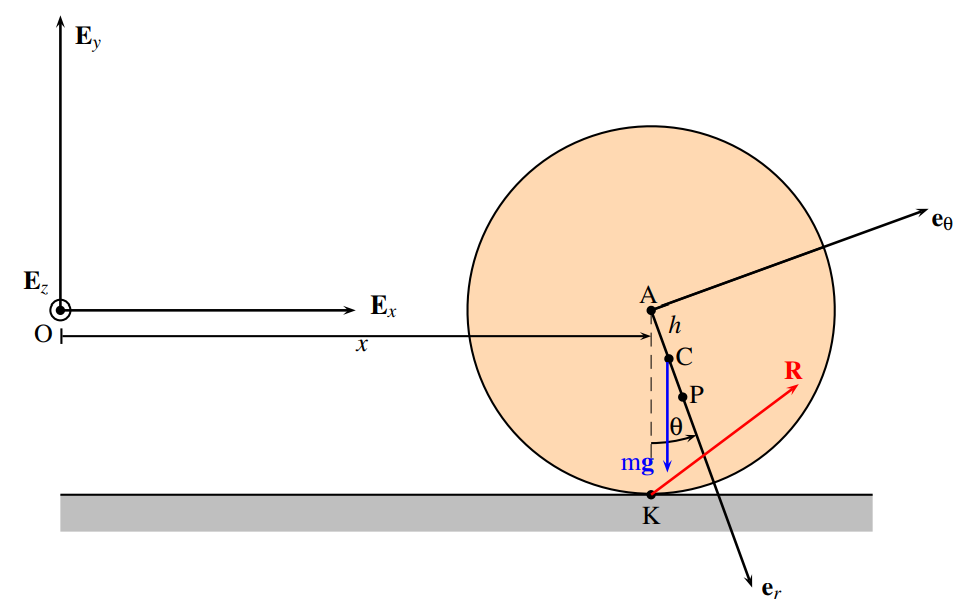
\includegraphics[width=0.5\textwidth]{images/SolideInertie.PNG}
\end{center}





\begin{enumerate}





%% Th. 1: théorème de la quantité de mouvement
\item Expression vectorielle du \textcolor{red}{\textbf{théorème de la quantité de mouvement}}\footnote{Explicitez chacune des résultantes cinématiques (pas leurs dérivées) et dynamiques intervenant dans ce théorème.}: Le théorème de la quantité de mouvement écrit au point \emph{O} donne:
\[ \dot{\textbf{N}}_O = \textbf{G} = m \textbf{g} + \textbf{R} \]
où: $\displaystyle \textbf{N}_O = m \; \dot{\textbf{s}}_C = m \frac{d}{d t} \big( x \; \textbf{E}_x + h \; \textbf{e}_r \big) = m \big( \dot{x} \; \textbf{E}_x + h \dot{\theta} \; \textbf{e}_\theta \big) $. \\
Dés lors, le théorème s'écrit: 
\[ m \frac{d}{d t} \big( \dot{x} \; \textbf{E}_x + h \dot{\theta} \; \textbf{e}_\theta \big) = m \textbf{g} + T \; \textbf{E}_x + N \; \textbf{E}_y \]





%% Th. 2: théorème du moment cinétique
\item Expression scalaire du \textcolor{red}{\textbf{théorème du moment cinétique}}\footnotemark[\value{footnote}] par rapport à un repère centré au centre d’inertie du solide et dont les axes sont parallèles à des axes inertiaux: Appliquant au solide étudié le théorème du moment cinétique rapporté à des axes parallèles aux axes absolus et centrés en \emph{C}, il vient:
\[ \dot{\textbf{H}}_C = \textbf{M}_C \]
où:
\[ \begin{aligned}
\textbf{M}_C &= \textbf{CC} \wedge m \textbf{g} + \textbf{CK} \wedge \textbf{R} = \big( -h \; \textbf{e}_r - a \; \textbf{E}_y \big) \wedge \big( N \; \textbf{E}_y + T \; \textbf{E}_x \big) \\
&= - h N \; (\textbf{e}_r \wedge \textbf{E}_y) - h T \; (\textbf{e}_r \wedge \textbf{E}_x) - a T \; (\textbf{E}_y \wedge \textbf{E}_x) \\
&= - h N \sin \theta \; \textbf{E}_z - h T \cos \theta \; \textbf{E}_z + a T \; \textbf{E}_z
\end{aligned} \]
et: $\displaystyle \textbf{H}_C = \textbf{J}_C \cdot \boldsymbol{\omega} = m b^2 \dot{\theta} \; \textbf{E}_z $, soit:
\[ \frac{d}{d t} \big( m b^2 \dot{\theta} \; \textbf{E}_z \big) = - h N \sin \theta \; \textbf{E}_z - h T \cos \theta \; \textbf{E}_z + a T \; \textbf{E}_z \]
ou encore, en projetant sur $ \textbf{E}_z $,
\[ \frac{d}{d t} \big( m b^2 \dot{\theta} \big) = - h N \sin \theta - h T \cos \theta + a T \]





%% Th. 3: théorème de l'énergie cinétique
\item \textcolor{red}{\textbf{Théorème de l’énergie cinétique}}\footnotemark[\value{footnote}] par rapport à un repère inertial: Le théorème de l’énergie cinétique rapporté à des axes inertiaux centrés en \emph{O}, s’écrit:
\[ \frac{d T_O}{d t} = \mathpzc{P}_O = m \textbf{g} \cdot \dot{\textbf{s}}_C + \textbf{R} \cdot \dot{\textbf{s}}_K = m \textbf{g} \cdot \dot{\textbf{s}}_C \]
vu la condition de roulement sans glissement et où: $\displaystyle T_O = \frac{1}{2} m \; \| \dot{\textbf{s}}_C \|^2 + T_C $ \\
avec: $ \| \dot{\textbf{s}}_C \|^2 = \dot{x}^2 + h^2 \dot{\theta}^2 + 2 h \dot{x} \dot{\theta} \cos \theta $ \\

et: $\displaystyle T_C = \frac{1}{2} \boldsymbol{\omega} \cdot \textbf{J}_C \cdot \boldsymbol{\omega} = \frac{1}{2} \dot{\theta} \; \textbf{E}_z \cdot \textbf{J}_C \cdot \dot{\theta} \; \textbf{E}_z = \frac{1}{2} m b^2 \dot{\theta}^2 $ \\
soit:
\[ \frac{1}{2} \frac{d}{d t} \bigg[ \frac{1}{2} m \big( \dot{x}^2 + h^2 \dot{\theta}^2 + 2 h \dot{x} \dot{\theta} \cos \theta + b^2 \dot{\theta}^2 \big) \bigg] = m \textbf{g} \cdot \dot{\textbf{s}}_C = - m g h \dot{\theta} \sin \theta \]





\end{enumerate}\section{Méthode Spécifique - Centre Géométrique} % Centre géométrique = Centre d'inertie





\begin{center}
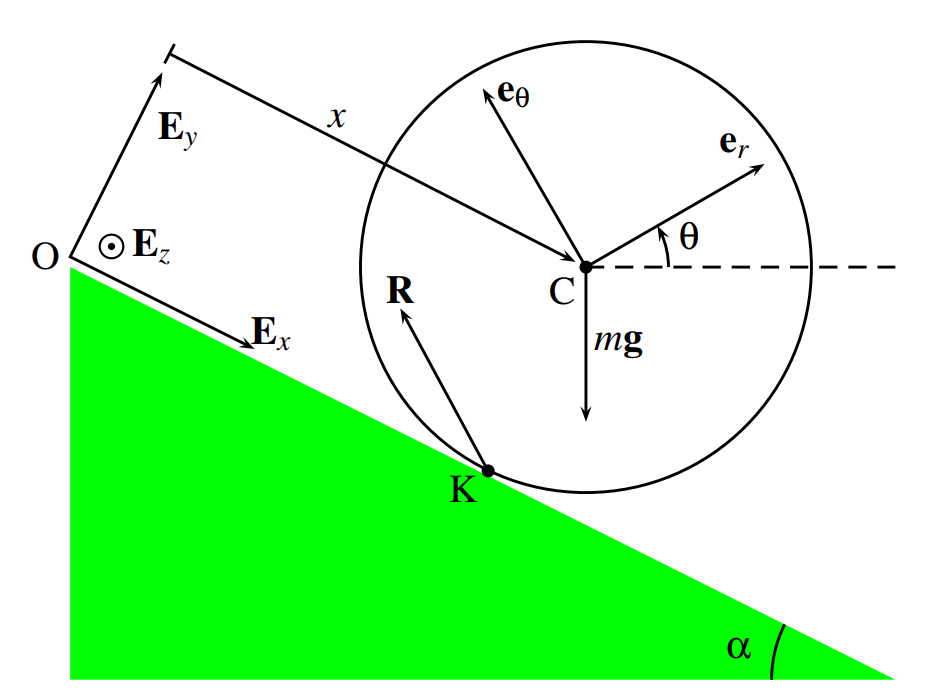
\includegraphics[width=0.6\textwidth]{images/SolideGeometrique.PNG}
\end{center}





\begin{enumerate}





%% Th. 1: théorème de la quantité de mouvement
\item Expression vectorielle du \textcolor{red}{\textbf{théorème de la quantité de mouvement}}\footnotemark[\value{footnote}]: Le théorème de la quantité de mouvement écrit au point \emph{O} donne:
\[ \dot{\textbf{N}}_O = \textbf{G} = m \textbf{g} + \textbf{R} \]
où: $\displaystyle \textbf{N}_O = m \; \dot{\textbf{s}}_C = m \dot{x} \; \textbf{E}_x $. \\
Dés lors, le théorème s'écrit: 
\begin{equation}\tag{Th.1}
m \ddot{x} \; \textbf{E}_x = m \textbf{g} + T \; \textbf{E}_x + N \; \textbf{E}_y 
\end{equation}





%% Th. 2: théorème du moment cinétique
\item Expression scalaire du \textcolor{red}{\textbf{théorème du moment cinétique}}\footnotemark[\value{footnote}] par rapport à un repère centré au centre d’inertie du solide et dont les axes sont parallèles à des axes inertiaux: Appliquant au solide étudié le théorème du moment cinétique rapporté à des axes parallèles aux axes absolus et centrés en \emph{C}, il vient:
\[ \dot{\textbf{H}}_C = \textbf{M}_C \]
où: $\displaystyle \textbf{M}_C = \textbf{CC} \wedge m \textbf{g} + \textbf{CK} \wedge \textbf{R} = - a \textbf{E}_y \wedge \big( T \; \textbf{E}_x + N \; \textbf{E}_y \big) = a T \; \textbf{E}_z $, et: $\displaystyle \textbf{H}_C = \textbf{J}_C \cdot \boldsymbol{\omega} = J_C \dot{\theta} \; \textbf{E}_z $, soit:
\begin{equation}\tag{Th.2}
J_C \ddot{\theta} = a T
\end{equation}





%% Th. 3: théorème de l'énergie cinétique
\item \textcolor{red}{\textbf{Théorème de l’énergie cinétique}}\footnotemark[\value{footnote}] par rapport à un repère inertial: Le théorème de l’énergie cinétique rapporté à des axes inertiaux centrés en \emph{O}, s’écrit:
\[ \frac{d T_O}{d t} = \mathpzc{P}_O = m \textbf{g} \cdot \dot{\textbf{s}}_C + \textbf{R} \cdot \dot{\textbf{s}}_K = m \textbf{g} \cdot \dot{\textbf{s}}_C \]
vu la condition de roulement sans glissement et où: $\displaystyle T_O = \frac{1}{2} m \; \| \dot{\textbf{s}}_C \|^2 + T_C $, avec: $ \| \dot{\textbf{s}}_C \|^2 = \dot{x}^2 $, et: $\displaystyle T_C = \frac{1}{2} \boldsymbol{\omega} \cdot \textbf{J}_C \cdot \boldsymbol{\omega} = \frac{1}{2} \dot{\theta} \; \textbf{E}_z \cdot \textbf{J}_C \cdot \dot{\theta} \; \textbf{E}_z = \frac{1}{2} J_C \dot{\theta}^2 $, soit:
\begin{equation}\tag{Th.3}
\frac{1}{2} \frac{d}{d t} \big( m \dot{x}^2 + J_C \dot{\theta}^2 \big) = m \dot{x} \; \ddot{x} + J_C \dot{\theta} \; \ddot{\theta} = m g \dot{x} \sin \alpha
\end{equation}





\end{enumerate}










\section{Méthode Générale - Suite}





\subsection{Indépendance des Équations}





Montrer que les équations découlant des théorèmes (Th.1, 2, 3) ne sont \textbf{pas} indépendantes.
\[ \begin{cases}
\ddot{x} \; \textbf{E}_x = m \textbf{g} + T \; \textbf{E}_x + N \; \textbf{E}_y \\
J_C \ddot{\theta} = a T \\
m \dot{x} \; \ddot{x} + J_C \dot{\theta} \; \ddot{\theta} = m g \dot{x} \sin \alpha
\end{cases} \]

Ici, on a trois méthodes: 
\begin{enumerate}

\item[(A)] On décrit comment on utilise les 2 premières équations pour arriver à la troisième: \\
Multipliant scalairement (Th.1) par: $ \dot{\textbf{s}}_C = \dot{x} \textbf{E}_x $, et lui ajoutant le produit de (Th.2) par: $ \dot{\theta} $, on obtient, en tenant compte de la condition de roulement sans glissement,
\[ m \dot{x} \; \ddot{x} + J_C \dot{\theta} \; \ddot{\theta} = (\dot{x} + a \dot{\theta}) T + m g \dot{x} \sin \theta = m g \dot{x} \sin \alpha \]
qui n’est autre que (Th.3). Les équations ne sont donc pas indépendantes.

\item[(B)] On remarque qu'on a trois équations pour trois inconnues (inconnues = $ \ddot{x}, T, N $) mais que quand on multiplie scalairement (Th.1) par: $ \textbf{E}_x $, on n'a plus qu'un système de trois équations à 2 inconnues.

\item[(C)] On écrit le système sous forme matricielle : \\
D'abord, on multiplie scalairement (Th.1) par $ \dot{x} \; \textbf{E}_x $, ce qui donne: $ \dot{x} \; \ddot{x} = m g \dot{x} \sin \alpha + \dot{x} T $
\[
\begin{pmatrix}
\dot{x} & - \dot{x} & 0 \\
-J_C/a & -a & 0 \\
m \dot{x} - J_C \dot{\theta}/a & 0 & 0
\end{pmatrix}
\begin{pmatrix}
\ddot{x} \\
T \\
N
\end{pmatrix}
=
\begin{pmatrix}
m g \dot{x} \sin \alpha \\
0 \\
m g \dot{x} \sin \alpha
\end{pmatrix}
\]
Étant donné qu'une des colonne de la matrice des coefficients est remplie de 0, on en conclu que le rang de cette matrice est inférieur à 3. Il y a donc une relation linéaire entre les lignes/colonnes de cette matrice. Les équations ne sont pas indépendantes.

\end{enumerate}





\subsection{Intégrales Premières}





On peut intégrer n'importe laquelle des équations que l'on a obtenue jusqu'à présent. Cependant, s'il faut choisir, autant prendre la troisième vu qu'il n'y a pas de \emph{T}.
\begin{equation}
m \dot{x} \; \ddot{x} + J_C \dot{\theta} \; \ddot{\theta} = m g \dot{x} \sin \alpha \tag{Th.3}
\end{equation}
On élimine la variable $ \theta $ avec la relation de roulement sans-glissement qu'on intègre pour obtenir:
\[ \frac{m \dot{x}^2}{2} \bigg( 1 + \frac{J_C}{m a^2} \bigg) = m g x \sin \alpha + C \]
On détermine la \textbf{constante d'intégration} grâce aux conditions initiales ($ C = 0 $). Ceci est l'intégrale première de \textcolor{red}{\textbf{conservation de l'énergie}}.

Si on avait intégré l'équation découlant du Th.1, l'intégrale première de conservation de la \textcolor{red}{\textbf{quantité de mouvement}}. \\
Et si on avait intégré l'équation découlant du Th.2, l'intégrale première de conservation du \textcolor{red}{\textbf{moment cinétique}}.

Dans ce système-ci, il n'y a pas conservation de ces grandeurs dynamiques car le solide prend de la vitesse et de la vitesse de rotation sans perdre de masse. La quantité de mouvement et la quantité de moment cinétique augmentent en fonction du temps au cours de cette phase de mouvement.

\textbf{Remarque}: Si on demande la loi de mouvement du solide, on doit dériver l'intégrale première puis la ré-intégrer 2 fois.





\subsection{Équation du Potentiel}





On peut aussi demander de montrer que le mouvement peut être étudié à partir d’une intégrale première du type: 
\[ f(\theta) \; \dot{\theta}^2 - 2 g h \cos \theta = C \]
où $ f(\theta) $ et \emph{C} sont à déterminer et désignent respectivement une fonction strictement positive et une constante.

C'est typiquement une intégrale première du Th.3 (théorème de l'énergie cinétique). En intégrant, on obtient donc: l’intégrale première de \textcolor{red}{\textbf{conservation de l’énergie}}. Une fois qu'on a intégré, on utilise la relation de roulement sans-glissement pour éliminer la variable \emph{x}. Il faut ensuite déterminer la constante d'intégration \emph{C} et la fonction $ f(\theta) $ en montrant que: $ f(\theta) > 0 $.





\subsection{Angle d'Inclinaison}





On demande souvent pour quelle angle $ \alpha $ la relation de roulement sans-glissement n'est plus valable.

Le roulement sans glissement est possible tant que $ | T | \leq \mu | N | $. Il faut utiliser l'équation du Th.1 pour obtenir la valeur de \emph{N} et le Th.2 pour obtenir \emph{T}. Ce qui nous permet d'écrire l'inégalité suivante:
\[ \text{const}_1 \; \sin \alpha \leq \mu \; \text{const}_2 \cos \alpha \]
\[ \tan \alpha \leq \mu \; \text{const}_3 \]










\section{Erreurs Fréquentes}





\begin{itemize}

\item Ne pas faire de dessin.

\item Ne pas bien orienter le repère lié au solide (pour la rotation). Pour rappel, l’angle $ \theta $ doit être mesuré à partir d’une direction fixe jusqu’au vecteur $ \textbf{e}_r $. Le vecteur $ \textbf{e}_\theta $ se trouve alors 90° plus loin que $ \textbf{e}_r $ dans la direction des $ \theta $ croissants qui doit être indiquée par une flèche.

\item Oublier le point P.

\item Calculer le tenseur par rapport à \emph{C} au lieu de la faire par rapport à \emph{O} (quand le point \emph{O} est fixe).

\item Mélanger tenseurs, vecteurs et scalaires et obtenir des expressions qui n’ont aucun sens mathématique.

\item Obtenir une expression dimensionnellement fausse et ne pas s’en rendre compte.

\item Oublier la force \emph{N}.

\item Croire que la force N est conservative.

\item Croire que l’absence de frottement implique que la force de liaison en ce point est horizontale (alors que cela indique juste l’absence d’un couple de réaction).

\item Ne pas souligner les vecteurs.

\item Ne pas savoir dériver la quantité de mouvement ou oublier de le faire.

\item Croire que $ \dot{\theta} = \omega_0 $ durant tout le mouvement.

\item Ne pas savoir calculer le moment cinétique.

\item Ne pas savoir dériver le moment cinétique ou oublier de le faire.

\item Ne pas savoir calculer le moment d’une force, en particulier inverser les termes dans le produit vectoriel.

\item Être incapable de calculer un produit vectoriel.

\item Croire que l’énergie cinétique et la puissance sont des vecteurs.

\item Ne pas savoir calculer l’énergie cinétique.

\item Ne pas savoir dériver l’énergie cinétique ou oublier de le faire.

\item Ne pas savoir calculer la puissance d’une force, en particulier, utiliser le vecteur position au lieu de la vitesse ou la même vitesse pour toutes les forces, malgré les points d’application différents. 
\item Être incapable de calculer correctement un produit scalaire.

\item Calculez une puissance nulle pour \textbf{N} et obtenir l’intégrale première de conservation de l’énergie.

\item Croire qu’au moment de l’impact, $ \ddot{\theta} = 0 $.

\item Essayer d’obtenir $ \dot{\theta} $ en intégrant l’expression de $ \ddot{\theta} $ avec \emph{N} considérée comme constante.

\item Introduire n’importe comment la force de liaison en \emph{O} à ce moment parce qu’on ne l’avait pas considérée au départ.

\item Obtenir une expression dimensionnellement fausse pour la force et ne pas s’en rendre compte.

\item Indiquer un angle $ \theta $ absolu sur son dessin (mesure par rapport à une direction fixe) et le considérer comme relatif dans le calcul des vitesses (et inversement).

\item Écrire les théorèmes au point \emph{O} qui n’est pas fixe.

\item Utiliser le théorème de transport pour obtenir le tenseur d’inertie en \emph{O'} à partir de celui en \emph{O}.

\end{itemize}




















\newpage




















\part{Annexe}










\section{Résolution d'Équations Différentielles Linéaires}





\begin{center} \begin{tikzpicture}[node distance = 2.cm]

\node (1) [cyan, yshift = 1.2cm, rounded corners] {\textbf{Équation différentielle}};
\node (2) [vert, fill = sprinen!65, below left of  = 1, yshift = -1cm, xshift = -2.5cm] {Premier degré};
\node (3) [vert, fill = sprinen!65, below right of = 1, yshift = -1cm, xshift = 2.5cm]  {Second degré \;};

\node (4) [rouge, below of = 2, draw = none, yshift  = -0.5cm] {Intégration directe};
\node (5) [rouge, below of = 3, draw = none, yshift  = -0.5cm] {Équation homogène};

\node (6) [rectangle, rounded corners, fill = yellow!30, below of = 4, draw = white, text width = 6cm]
{$\displaystyle \big[I(x) = e^{\int P(x) d x} \times \big] \; y' + P(x) y = Q(x) $ \\
$\displaystyle \implies y = \frac{1}{I(x)} \Big[ \int I(x) Q(x) \; d x + C \Big] $};
\node (7) [rectangle, rounded corners, fill = blue!30, below of = 6, draw = white] {$\displaystyle y' + a x = b \implies y(x) = \frac{b}{a} + C_1 \; e^{-a x} $};

\node (8) [rectangle, rounded corners, fill = yellow!30, below of = 5, draw = white, text width = 6cm]
{Racines de $ a r^2 + b r + c = 0 $ : \\
$ (1) \; r_1 $ et $ r_2 $ réelles et distinctes \\
$ (2) \; r_1 = r_2 = r $ \\
$ (3) \; r_1 $, $ r_2 $ complexes : $ \alpha \pm i \beta $};

\node (9) [rectangle, rounded corners, fill = blue!30, yshift = 0cm, below of = 8, draw = white, text width = 6cm]
{$\displaystyle (1) \; y = C_1 e^{r_1 x} + C_2 e^{r_2 x} $ \\
$\displaystyle (2) \; y = C_1 e^{rx} + C_2 x e^{rx} $ \\
$\displaystyle (3) \; y = e^{\alpha x} (C_1 \cos \beta x + C_2 \sin \beta x) $};

\node (10) [vert, fill = sprinen!65, below of = 1, yshift  = -0.5cm] {Degré supérieur};
\node (11) [rectangle, rounded corners, fill = yellow!30, below of = 10, draw = white, text width = 12cm, yshift = -7cm]
{\[ y^{(n)} + a_{n-1} \; y^{(n-1)} + ... + a_1 \; y' + a_0 \; y = 0 \]
$\displaystyle \implies y = C_1 e^{\lambda_1 x} + C_2 e^{\lambda_2 x} + ... + (C_n + C_{n+1} x + ... + C_{n+\alpha} x^\alpha) e^{\lambda_n x} $ \\
où $ \lambda_n $ est de multiplicité $ \alpha $};

\draw[->] (1) -- (2);
\draw[->] (1) -- (3);
\draw[->] (1) -- (10);

\draw[->] (2) -- (4);
\draw[->] (3) -- (5);
\draw[->] (4) -- (6);
\draw[->] (6) -- (7);

\draw[->] (5) -- (8);
\draw[->] (8) -- (9);

\draw[->] (10) -- (11);

\end{tikzpicture} \end{center}

Si l'équation n'est pas homogène mais que les coefficients sont constants, on utilise la méthode des coefficients indéterminés, c-à-d : lorsque l'équation différentielle est du type $ a y'' + b y' + c y = G(x) $ : 
\begin{center} \begin{tabular}{p{6cm}p{6cm}}
\hline
$ G(x) $ & À remplacer dans l'équa. diff. \\
\hline
$ G(x) = P(x) $ & $ Y_P = Q(x) $ \\
$ G(x) = e^{k x} P(x) $ & $ Y_P = e^{k x} Q(x) $ \\
$ G(x) = e^{k x} P(x) \cos m x $ & $ Y_P = e^{k x} Q(x) \cos m x + e^{k x} R(x) \sin m x $ \\
\hline
\end{tabular} \end{center}
où $ P(x) $ et $ Q(x) $ sont des polynômes du style de $ a x^2 + b x + c $. \\
Remarques : 

\begin{itemize}
\item $ A \cos m x + B \sin m x = C \cos ( m x + \varphi_1 ) = C \sin ( m x + \varphi_2 ) $.
\item Si $ Y_P(x) $ est une solution de l'équation homogène, alors on remplace $ Y_P(x) $ par $ x Y_P(x) $.
\end{itemize}










\section{Variables Adimensionnelles}





Le changement de variable : $\displaystyle \tau = \frac{t}{t^*} $, permet d'écrire : 
\[ \frac{d}{d t} = \frac{d}{d \tau} \frac{d \tau}{d t} = \frac{1}{t^*} \frac{d}{d \tau} = \frac{1}{t^*} ( \; \mathring{} \; ) \]










\section{Loi de Newton dans un Repère Non-Inertiel}





Lorsqu'on est dans un repère non-inertiel, une décomposition de l'accélération peut être effectuée : 
\[ \frac{d^2 \textbf{s}}{d t^2} = \underbrace{ \frac{d^2 \textbf{b}}{d t^2} + \dot{\textbf{w}} \wedge \textbf{r} + \textbf{w} \wedge (\textbf{w} \wedge \textbf{r}) }_{\textbf{a}_e} + \underbrace{ 2 \; \textbf{w} \wedge \frac{\delta \textbf{r}}{\delta t} }_{\textbf{a}_c} + \underbrace{ \frac{\delta^2 \textbf{r}}{\delta t^2} }_{\textbf{a}_r} \]
où $ \textbf{a}_e $ est l'accélération d'entraînement, $ \textbf{a}_c $ est l'accélération de Coriolis et $ \textbf{a}_r $ est l'accélération relative.

La \textcolor{red}{\textbf{Loi de Newton}} (équation différentielle vectorielle du mouvement) qui devrait s'écrire : 
\[ \textbf{F} = m \; \ddot{\textbf{s}} \qquad \qquad \qquad \sum \textbf{F}_{\text{extérieures}} = m \; \ddot{\textbf{s}} \]
S'écrit, dans un repère non-inertiel : 
\[ \begin{aligned} m \; \textbf{a}_r = m \frac{\delta^2 \textbf{r}}{\delta t^2} &= \textbf{G} - m \; \textbf{a}_e - m \; \textbf{a}_c \\ &= \textbf{G} - m \Big[ \frac{d^2 \textbf{b}}{d t^2} + \dot{\textbf{w}} \wedge \textbf{r} + \textbf{w} \wedge (\textbf{w} \wedge \textbf{r}) \Big] - m \Big[ 2 \textbf{w} \wedge \frac{\delta \textbf{r}}{\delta t} \Big] \end{aligned} \]










\section{Stabilité et Dérivées}





\begin{itemize}


%% Rappel : extrema d'une fonction
\item Rappel : Extrema d'une fonction : \\
Si \emph{f} est une fonction réelle $ n + 1 $ fois continûment dérivable sur $ ]a, b[ $, si $ f'(c) = 0 $ en un point $ c \in \; ]a, b[ $ et si la première dérivée non-nulle en \emph{c} est $ f^{(n)} (c) $, alors : 
\begin{itemize}
\item[--] \emph{c} est un maximum local si \emph{n} est pair et $ f^{(n)}(c) < 0 $.
\item[--] \emph{c} est un minimum local si \emph{n} est pair et $ f^{(n)}(c) > 0 $.
\item[--] \emph{c} est un point d'inflexion à tangente horizontale si \emph{n} est pair.
\end{itemize}





%% Types d'équilibre
\item Pour rappel, on a 4 types "d'équilibres" : Stable, Instable, Marginalement Stable, Faiblement Instable. \\
Et par exemple, si on a une équation différentielle linéaire à coefficients constants dont on veut connaître la stabilité : 

\begin{center} \begin{tabular}{|p{6cm}|p{8cm}|} \hline
Racines du polynôme caractéristique : $ z_1 = a_1 + i b_1 \; \; \text{et} \; \; z_2 = a_2 + i b_2 $ & Stabilité : méthode des perturbations infinitésimales (éq. linéaire) \\ \hline
$ a_1 < 0 $ et $ a_2 < 0 $ & Équilibre \textbf{stable}
\[ x(t) = C_1 e^{- x t} + C_2 e^{- y t} \] \\ \hline
Si $ a_1 > 0 $ ou $ a_2 > 0 $ & Équilibre \textbf{instable}
\[ x(t) = C'_1 e^{\alpha t} + C'_2 e^{- \alpha t} = C_1 \text{ sh } \alpha t + C_2 \text{ ch } \alpha t \] \\ \hline
$ a_1 < 0, \; a_2 = 0 $ \; ou \; $ a_1 = 0, \; a_2 < 0  $ \; \danger avec $ k = 0 $ \quad (k = multiplicité) & Équilibre \textbf{marginalement stable}, \[ x(t) = C'_1 e^{i \alpha t} + C'_2 e^{- i \alpha t} \; = C_1 \sin \alpha t + C_2 \cos \alpha t \] \\ \hline
$ z_1 = z_2 = 0 $ \qquad ($ k \neq 0 $) & Équilibre \textbf{faiblement instable} \[ x(t) = A t + B \] \\ \hline
\end{tabular} \end{center}


\end{itemize}










\section{Grandeurs Caractéristiques}





Voici des grandeurs globales représentatives de l’ensemble du système : 
\begin{center} \begin{tabular}{|c|c|} \hline
Masse totale : $\displaystyle m = \int d m $ & Moment statique : $\displaystyle \textbf{Q}_O = \int \textbf{s} \; d m $ \\ \hline
Quantité de mouvement : $\displaystyle \textbf{N}_O = \int \dot{\textbf{s}} \; d m $ & Résultante des forces : $\displaystyle \textbf{G} = \int \textbf{F} \; d m $ \\ \hline
Moment cinétique : $\displaystyle \textbf{H}_O = \int \textbf{s} \wedge \dot{\textbf{s}} \; d m $ & Moment dynamique : $\displaystyle \textbf{M}_O = \int \textbf{s} \wedge \textbf{F} \; d m $ \\ \hline
Énergie cinétique : $\displaystyle T_O = \frac{1}{2} \int \dot{\textbf{s}} \cdot \dot{\textbf{s}} \; d m $ & Puissance : $\displaystyle \mathpzc{P} = \int \dot{\textbf{s}} \cdot \textbf{F} \; d m $ \\ \hline  \end{tabular} \\
Remarque: ici, \textbf{F} correspond à l'accélération $ \ddot{\textbf{s}} $.
\end{center}





Théorèmes généraux en mécanique du solide : 
\begin{itemize}





%% Théorème de la quantité de mouvement
\item Théorème de la quantité de mouvement (Th. I) : 
\begin{center}
\ovalbox {\begin{minipage}{0.93\textwidth}
Dans un repère inertiel, la dérivée temporelle de la quantité de mouvement d'un système matériel est égale à la résultante des forces extérieures qui lui sont appliquées : 
\[ \frac{d \textbf{N}_O}{d t} = \textbf{G} \]
\end{minipage}}
\end{center}
Ce qui implique que le centre d'inertie d'un système (de masse m) "agit" comme un point matériel de masse m soumis à la résultante des forces extérieures ($ m \; \ddot{\textbf{c}} = \textbf{G} $).





%% Théorème du moment cinétique
\item Théorème du moment cinétique (Th. II) : 
\begin{center}
\ovalbox {\begin{minipage}{0.93\textwidth}
Dans un repère inertiel, la dérivée temporelle du moment cinétique d'un système matériel par rapport à un point fixe O est égale à la résultant des moments par rapport à ce point des forces extérieures appliquées au système : 
\[ \dot{\textbf{H}}_O = \textbf{M}_O \]
\end{minipage}}
\end{center}





%% Théorème de l'énergie cinétique
\item Théorème de l'énergie cinétique (Th. III) : 
\begin{center}
\ovalbox {\begin{minipage}{0.93\textwidth}
Dans un repère inertiel, la puissance développée par l'ensemble des forces intérieures appliquées à un système matériel est égale à la dérivée temporelle de son énergie cinétique : 
\[ \dot{T}_O = \mathpzc{P}_O \]
\end{minipage}}
\end{center}

\end{itemize}










\section{Théorème C et Implications}





%% Théorème C
Théorème C : 
\begin{center}
\ovalbox {\begin{minipage}{0.93\textwidth}
Chacune des résultantes, calculée dans le système d'axes de centre O, est égale à la même résultante, calculée dans le système d'axes parallèles de centre C, augmentée de la résultante correspondante du centre d'inertie considéré comme un point matériel affecté de la masse totale du système et soumis à la résultante des forces.
\end{minipage}}
\end{center}



%% Conclusions du théorème C
Le théorème C nous permet d'écrire : \\
\begin{tabular}{p{0.45\textwidth}p{0.45\textwidth}}
\begin{itemize}
\item $ \textbf{Q}_O = m \textbf{c} + \textbf{Q}_C $
\item $ \textbf{N}_O = m \dot{\textbf{c}} + \textbf{N}_C $
\item $ \textbf{H}_O = m \textbf{c} \wedge \dot{\textbf{c}} + \textbf{H}_C $
\end{itemize} & 
\begin{itemize}
\item $\displaystyle T_O = \frac{1}{2} m \| \dot{\textbf{c}} \|^2 + T_C $
\item $ \textbf{M}_O = \textbf{c} \wedge \textbf{G} + \textbf{M}_C $
\item $ \mathpzc{P}_O = \dot{\textbf{c}} \cdot \textbf{G} + \mathpzc{P}_C $
\end{itemize} \end{tabular}


%% Grandeurs résultantes du solide
Grandeurs résultantes du solide : \\
Si l'on définit le tenseur central d'inertie $\textbf{J}_C $ d'un solide par rapport au point C (référentiel d'origine C) quelconque du solide par l'expression : $\displaystyle \textbf{J}_C = \int ( r^2 \textbf{I} - \textbf{r} \; \textbf{r} ) \; d m $, alors on a : \\
\begin{tabular}{p{0.45\textwidth}p{0.45\textwidth}}
\begin{itemize}
\item $\displaystyle \textbf{H}_C = \textbf{J}_C \cdot \textbf{w} $
\item $\displaystyle T_C = \frac{1}{2} \textbf{w} \cdot \textbf{H}_C = \frac{1}{2} \textbf{w} \cdot \textbf{J}_C \cdot \textbf{w} $
\item $\displaystyle \textbf{Q}_C = \textbf{N}_C = \textbf{0} $
\end{itemize} & 
\begin{itemize}
\item $\displaystyle \textbf{M}_C = \int (\textbf{r} \wedge \hat{\textbf{F}}) \; d m $
\item $\displaystyle \mathpzc{P}_C = \textbf{w} \cdot \textbf{M}_C $
\end{itemize} \end{tabular} \\
De manière générale, on prend le centre d'inertie comme point C pour simplifier les calculs. Et pour rappel, \textbf{w} est le vecteur de Poisson.


%% Preuve que $ \textbf{H}_C = \textbf{J}_C \cdot \textbf{w} $
Preuve que $ \textbf{H}_C = \textbf{J}_C \cdot \textbf{w} $ : 
D'abord, remarquons que $\displaystyle \dot{\boldsymbol{\sigma}} = \textcolor{red}{\cancel{\frac{\delta \boldsymbol{\sigma}}{\delta t}}} + \textbf{w} \wedge \boldsymbol{\sigma} $.
\begin{center} 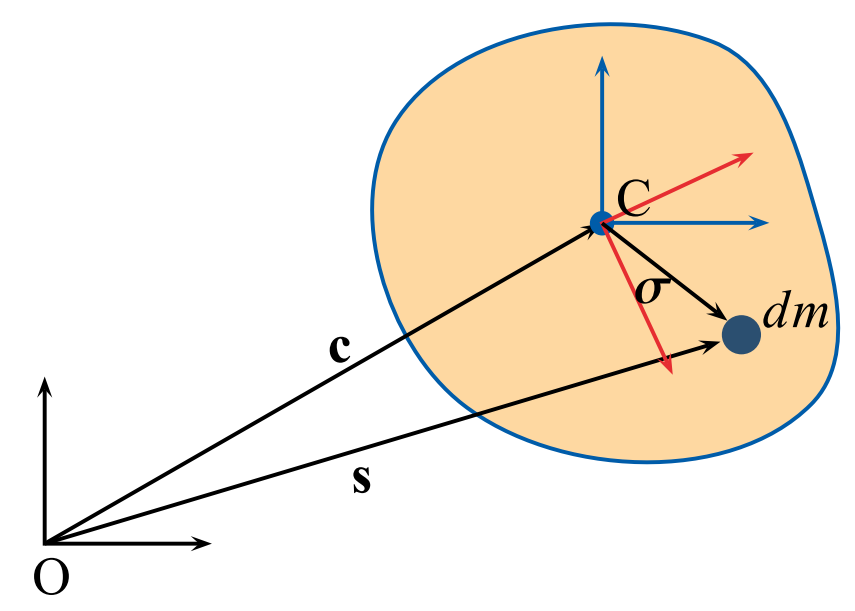
\includegraphics[width=0.4\textwidth]{images/Solide.PNG} \end{center}
\begin{align*}
\textbf{H}_C &= \int \boldsymbol{\sigma} \wedge \dot{\boldsymbol{\sigma}} \; d m \\
&= \int \boldsymbol{\sigma} \wedge ( \textbf{w} \wedge \boldsymbol{\sigma} ) \; d m \qquad \qquad \textbf{a} \wedge (\textbf{b} \wedge \textbf{c}) = \textbf{b} (\textbf{a} \cdot \textbf{c}) - \textbf{c} (\textbf{a} \cdot \textbf{b}) \\
&= \int \textbf{w} \| \boldsymbol{\sigma} \|^2 - \boldsymbol{\sigma} (\boldsymbol{\sigma} \cdot \textbf{w}) \; d m \\
&= \int ( \| \boldsymbol{\sigma} \|^2 \textbf{I} - \boldsymbol{\sigma} \; \boldsymbol{\sigma} ) \cdot \textbf{w} \; d m = \textbf{w} \cdot \int ( \| \boldsymbol{\sigma} \|^2 \textbf{I} - \boldsymbol{\sigma} \; \boldsymbol{\sigma} ) \; d m \\
&= \textbf{J}_C \cdot \textbf{w} \qquad \qquad \text{ où } \textbf{J}_C = \int ( \| \boldsymbol{\sigma} \|^2 \textbf{I} - \boldsymbol{\sigma} \; \boldsymbol{\sigma} ) \; d m
\end{align*}











\section{Rappel}





\begin{itemize}

\item La dérivée de : $ \textbf{e}_r $, est donnée par : $ \dot{\textbf{e}}_r = \dot{\theta} \; \textbf{e}_\theta $.

\item La dérivée de : $ \textbf{e}_\theta $, est donnée par : $ \dot{\textbf{e}}_\theta = - \dot{\theta} \; \textbf{e}_r $.

\end{itemize}










\section{Roulement Sans-Glissement}





\begin{center} 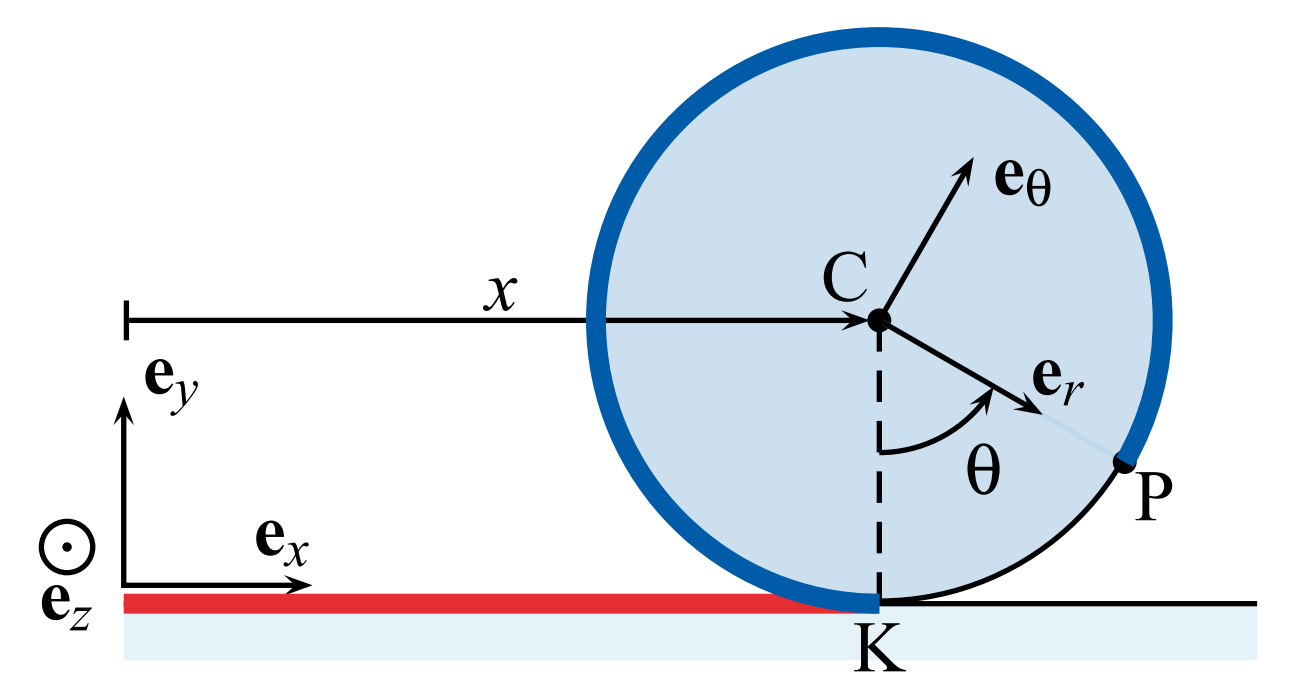
\includegraphics[width=0.6\textwidth]{images/Solides3.PNG} \end{center}

On veut exprimer la vitesse de $ \dot{\textbf{s}}_K ( = \textbf{0}) $ en \textbf{passant par son centre d'inertie}.
\begin{enumerate}

\item On essaie de trouver la position d'un point quelconque de la périphérie en passant par son centre d'inertie. \\
\textbf{Attention}, on utilise un repère absolu pour donner la coordonnée du centre d'inertie \emph{C}.

\item On veut décrire l'orientation du solide dans l'espace. Pour cela, il suffit de donner un angle $ \theta $ qui décrive la rotation de la roue autour de son centre, autour de l'axe.

\item L'angle $ \theta $ (qui décrit la rotation du solide) est toujours un angle qui est pris par rapport à une \textbf{direction fixe} et qui pointe vers une direction variable liée au solide.

\item Une fois qu'on a la position du point ainsi décrite, on peut la dériver pour avoir la vitesse qu'on égale à \textbf{0} pour avoir notre \emph{bonne vieille} condition de roulement sans-glissement.

\end{enumerate}


Dans le cas de la roue (rayon = \emph{a}) ci-dessus, on a 2 méthodes: 
\begin{enumerate}[label=(\Alph*)]
\item Première Méthode:
\[ \textbf{s}_K = \underbrace{x \; \textbf{E}_x + R \; \textbf{E}_y}_{\textbf{c}} + a \; \textbf{e}_r \implies \dot{\textbf{s}}_K = \dot{x} \; \textbf{E}_x + a \dot{\theta} \; \textbf{e}_\theta \]
\[ \fbox{$ \dot{x} + a \dot{\theta} = 0 $} \]
\item Seconde Méthode:
\[ \dot{\textbf{s}}_K = \dot{x} \; \textbf{E}_x + \underbrace{\dot{\theta} \; \textbf{E}_z}_{\boldsymbol{\omega}} \wedge \textbf{CK} = \dot{x} \; \textbf{E}_x + \dot{\theta} \; \textbf{E}_z \wedge (- a \; \textbf{E}_y) = \dot{x} \; \textbf{E}_x + a \dot{\theta} \; \textbf{E}_x \]
\[ \fbox{$ \dot{x} + a \dot{\theta} = 0 $} \]

\end{enumerate}










\section{Calcul Moments d'Inertie Fréquents}





\begin{enumerate}

\item[(a)] \textcolor{red}{\textbf{Système rectiligne}} : Il suffit de calculer un seul moment d'inertie par rapport à une droite perpendiculaire à la droite du solide.

\item[(b)] \textcolor{red}{\textbf{Système plan}} : (plan $ Oxy $, $ z = 0 $)
\[ J_x = \int y^2 \; d m \qquad ; \qquad J_y = \int x^2 \; d m \qquad ; \qquad J_z = \int \Big( x^2 + y^2 \Big) \; d m \]
Et donc : $\displaystyle J_x + J_y = J_z $

\end{enumerate}





Théorèmes particuliers en rapport avec le tenseur d'inertie : 
\begin{enumerate}

\item[(c)] \textcolor{red}{\textbf{Théorème C}} : 
\[ \textbf{J}_O = \textbf{J}_C + m \; \Big[ c \; \textbf{I} - \textbf{c} \textbf{c} \Big] \]

\item[(d)] Le \textcolor{red}{\textbf{théorème de transport}} est un théorème qui donne le moment d'inertie autour d'une droite $ d_1 $ passant par \emph{O} parallèle à $ d_2 $ passant par \emph{C} : $\displaystyle J_O^{d_1} = J_C^{d_2} + m l^2 $.

\item[(e)] Ce qu'on veut souvent calculer, c'est le $ J_C $ d'un \textcolor{red}{\textbf{mouvement plan}}. Il vaut: 
\[ J_C = \int (x^2 + y^2) \; d m = \int x^2 \; d m + \int y^2 \; d m \]

\item[(f)] \textbf{Moments d'inertie de base}:
\begin{itemize}
    \item Tige rectiligne: $\displaystyle J_C = \frac{1}{12} m l^2 $
    \item Anneau (cercle): $\displaystyle J_C = m r^2 $
    \item Disque plein: $\displaystyle J_C = \frac{1}{2} m r^2 $
    \item Rectangle plein: $\displaystyle J_C = \frac{1}{12} m (l^2 + h^2) $
\end{itemize}

\end{enumerate}










\section{Forces Surfaciques}





\begin{center} 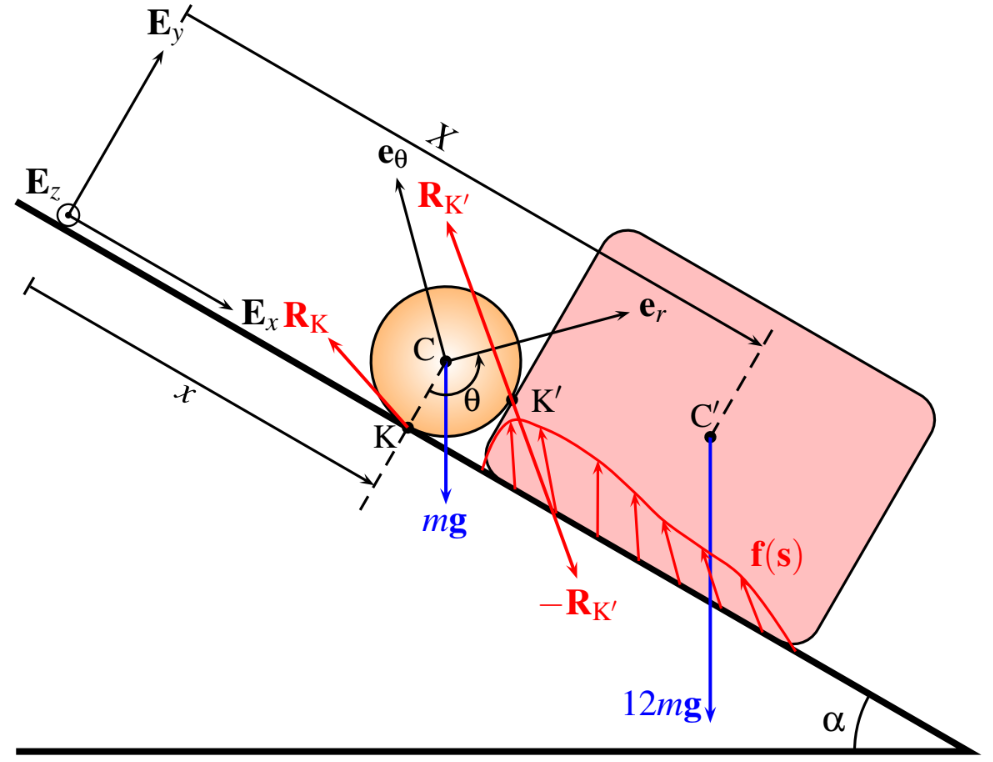
\includegraphics[width=0.5\textwidth]{images/ForceSurfacique.PNG} \end{center}

Ici, la force $ \textbf{f}(\textbf{s}) $ agissant sur le casier est une force surfacique. si on a ça à un examen, il faut noter: \\
$ \textbf{f}(\textbf{s}) $: distribution surfacique de forces de liaison agissant sur la surface $ \Sigma $ du casier en contact avec le plan, de direction inconnue dans le plan du mouvement. Notons $ \textbf{R} = \textbf{N} + \textbf{T} = N \textbf{E}_y + T \textbf{E}_x $ la résultante de cette distribution.










\newpage










\section{Examens}





La théorie couvre tous les examens (jusque janvier 2019).

Examens avec Q. sur les \textcolor{blue}{\textbf{forces centrales}}, examens avec Q. sur les \textcolor{red}{\textbf{solides qui roulent}}:
\begin{itemize}

\item Janvier 2011: 1 question - \textcolor{red}{\textbf{solide qui roule}}

\item Août 2011: Q1 - similaire à la méthode des \textcolor{blue}{\textbf{forces centrales}}, Q2 - \textcolor{violet}{\textbf{moment d'inertie}} + \textcolor{violet}{\textbf{pendule}}

\item Janvier 2012: Q1 - \textcolor{blue}{\textbf{force centrale}}, Q2 - \textcolor{violet}{\textbf{pendule}}

\item Août 2012: Q1 - \textcolor{red}{\textbf{solide qui roule}}, Q2 - \textcolor{violet}{\textbf{moment d'inertie}} + \textcolor{violet}{\textbf{pendule}}

\item Janvier 2013: Q1 - \textcolor{blue}{\textbf{force centrale}}, Q2 - \textcolor{violet}{\textbf{moment d'inertie}} + \textcolor{violet}{\textbf{pendule}}

\item Août 2013: Q1 - \textcolor{violet}{\textbf{courbe de guidage fixe}}, Q2 - \textcolor{violet}{\textbf{pendule}}

\item Janvier 2014: Q1 - \textcolor{violet}{\textbf{courbe de guidage mobile}} + \textcolor{violet}{\textbf{pendule}} - système similaire à septembre 2017, Q2 - théorie

\item Août 2014: Q1 - théorie, Q2 - \textcolor{blue}{\textbf{force centrale}}, Q3 - \textcolor{red}{\textbf{solide qui roule}}

\item Janvier 2015: Q1 - théorie, Q2 - \textcolor{violet}{\textbf{courbe de guidage mobile}}, Q3 - \textcolor{red}{\textbf{solide qui roule}}

\item Août 2015: Q1 - théorie, Q2 - \textcolor{violet}{\textbf{courbe de guidage mobile}}, Q3 - \textcolor{red}{\textbf{solide qui roule}} (Relire quand même)

\item Janvier 2016: Q1 - théorie, Q2 - \textcolor{blue}{\textbf{force centrale}}, Q3 - \textcolor{violet}{\textbf{moment d'inertie}} + \textcolor{violet}{\textbf{point fixe}}

\item Août 2016: Q1 - théorie, Q2 - \textcolor{violet}{\textbf{masse variable}}, Q3 - \textcolor{red}{\textbf{solide qui roule}}

\item Janvier 2017: Q1 - théorie, Q2 - \textcolor{blue}{\textbf{force centrale}}, Q3 - \textcolor{red}{\textbf{solide qui roule}}

\item Août 2017: Q1 - théorie, Q2 - \textcolor{violet}{\textbf{courbe de guidage mobile}}, Q3 - \textcolor{red}{\textbf{solide qui roule}} + \textcolor{violet}{\textbf{courbe de guidage fixe}} (Relire exercice dirigé 2017)

\item Janvier 2018: Q1 - théorie, Q2 - similaire à la méthode des \textcolor{blue}{\textbf{forces centrales}}, Q3 - \textcolor{red}{\textbf{solide qui roule}} + \textcolor{violet}{\textbf{moment d'inertie}}

\item Août 2018: Q1 - théorie, Q2 - \textcolor{blue}{\textbf{forces centrales}}, Q3 - \textcolor{red}{\textbf{solide qui roule}}

\end{itemize}


Il faudrait refaire un truc sur les pendules.










\section{Exemple: calcul du moment d'inertie}





\begin{center} 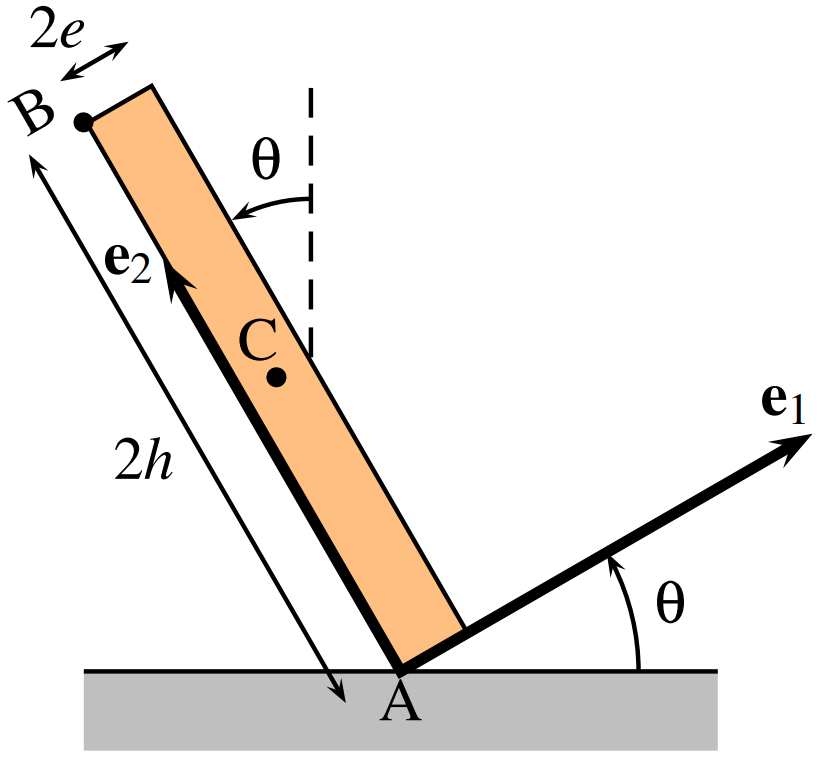
\includegraphics[width=0.4\textwidth]{images/ExMomentInertie.PNG} \end{center}

\begin{siderules} Montrez, en repartant de la définition des moments d’inertie, que le moment d’inertie du domino pour la rotation autour de A dans le plan du mouvement est donné par
\[ J_A = \frac{4}{3} m (e^2 + h^2) \] \end{siderules}


\textbf{Méthode n°1}: Par définition, le moment d’inertie recherché est donné par
\[ J_A = \int_0^{2h} d y \int_0^{2e} \rho l (x^2 + y^2) \; d x = \rho l \int_0^{2h} \bigg[ \frac{x^3}{3} + y^2 x \bigg] \; d y = \frac{16}{3} \rho l e h (e^2 + h^2) \]
où \emph{l} est l'épaisseur du solide et $ \rho $ la masse par unité de volume. Puisque $ m = 4 \rho l e h $, il vient: 
\[ J_A = \frac{4}{3} m (e^2 + h^2) \]

\textbf{Méthode n°2}: Le moment d'inertie de base d'un rectangle plein est donné par $ J_C = m (l^2 + h^2) / 12 $, dans notre cas, la largeur et la longueur valent $ 2 e $ et $ 2 h $. D'où, $ J_C = 1/3 \times m (e^2 + h^2) $. Le théorème de transport nous permet finalement d'arriver à: 
\[ J_C = \frac{1}{3} m (e^2 + h^2) + m (e^2 + h^2) = \frac{4}{3} m (e^2 + h^2) \]










\section{Mouvement du Solide autour d'un Point Fixe}





\begin{center} 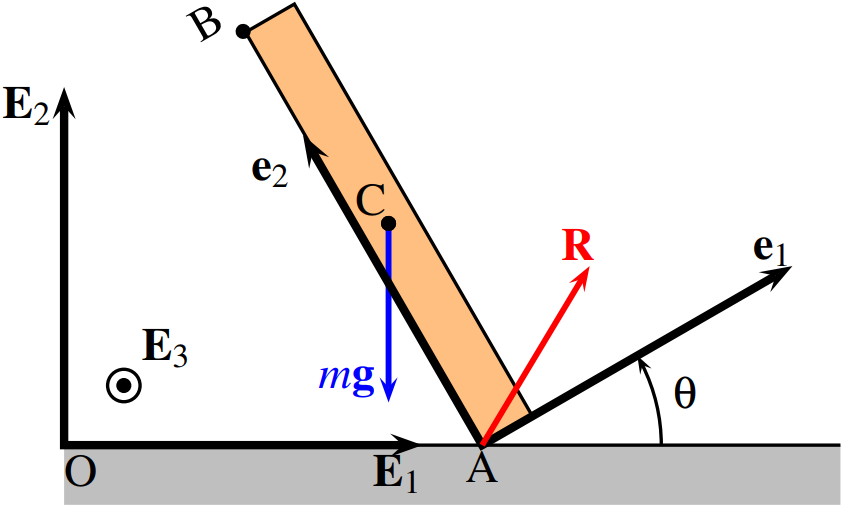
\includegraphics[width=0.5\textwidth]{images/MouvementPointFixe.PNG} \end{center}

\begin{siderules}
Exprimez la vitesse et l’accélération absolues du centre d’inertie C dans les axes $ \textbf{e}_1, \textbf{e}_2 $ liés au solide.
\end{siderules}

On a: 
\[ \begin{aligned}
\textbf{c} &= e \; \textbf{e}_1 + h \; \textbf{e}_2 \\
\dot{\textbf{c}} &= e \dot{\theta} \textbf{E}_3 \wedge \textbf{e}_1 + h \dot{\theta} \textbf{E}_3 \wedge \textbf{e}_2 = e \dot{\theta} \textbf{e}_2 - h \dot{\theta} \textbf{e}_1 \\
\ddot{\textbf{c}} &= (- h \ddot{\theta} - e \dot{\theta}^2) \textbf{e}_1 + (e \ddot{\theta} - h \dot{\theta}^2) \textbf{e}_2
\end{aligned} \]
en tenant compte du fait que le vecteur de Poisson du domino et des axes $ \textbf{e}_1 $ et $ \textbf{e}_2 $ qui y sont attachés est: $ \boldsymbol{\omega} = \dot{\theta} \textbf{E}_3 $.




Le \textbf{moment cinétique} en A est donné par: $\displaystyle \textbf{H}_A = J_A \dot{\theta} \textbf{E}_3 $.

Le \textbf{théorème du moment cinétique} rapporté à des axes absolus centrés en A s'écrit donc: $\displaystyle \dot{\textbf{H}}_A = \textbf{c} \wedge m \textbf{g} + \textbf{0} \wedge \textbf{R} \implies J_A \ddot{\theta} = - m g e \cos \theta + m g h \sin \theta $.









\newpage










\tableofcontents






























\end{document}





















































































%%%%%%%%%%%%%%%%%%%%%%%%%%%%%%%%%%%%%%%%%%%%%%%%%%%%%%%%%%%%%%%%%%%%%%%%%%%%%%%%%%%%%%%%%
%%%%%%%%%%%%%%%%%%%%%%%%%%%%%%%%%%%%%%%%%%%%%%%%%%%%%%%%%%%%%%%%%%%%%%%%%%%%%%%%%%%%%%%%%
%%%%%%%%%%%%%%%%%%%%%%%%%%%%%%%%%%%%%%%%%%%%%%%%%%%%%%%%%%%%%%%%%%%%%%%%%%%%%%%%%%%%%%%%%
%%%%%%%%%%%%%%%%%%%%%%%%%%%%%%%%%%%%%%%%%%%%%%%%%%%%%%%%%%%%%%%%%%%%%%%%%%%%%%%%%%%%%%%%%
%%%%%%%%%%%%%%%%%%%%%%%%%%%%%%%%%%%%%%%%%%%%%%%%%%%%%%%%%%%%%%%%%%%%%%%%%%%%%%%%%%%%%%%%%
%%%%%%%%%%%%%%%%%%%%%%%%%%%%%%%%%%%%%%%%%%%%%%%%%%%%%%%%%%%%%%%%%%%%%%%%%%%%%%%%%%%%%%%%%
%%%%%%%%%%%%%%%%%%%%%%%%%%%%%%%%%%%%%%%%%%%%%%%%%%%%%%%%%%%%%%%%%%%%%%%%%%%%%%%%%%%%%%%%%
%%%%%%%%%%%%%%%%%%%%%%%%%%%%%%%%%%%%%%%%%%%%%%%%%%%%%%%%%%%%%%%%%%%%%%%%%%%%%%%%%%%%%%%%%
%%%%%%%%%%%%%%%%%%%%%%%%%%%%%%%%%%%%%%%%%%%%%%%%%%%%%%%%%%%%%%%%%%%%%%%%%%%%%%%%%%%%%%%%%
%%%%%%%%%%%%%%%%%%%%%%%%%%%%%%%%%%%%%%%%%%%%%%%%%%%%%%%%%%%%%%%%%%%%%%%%%%%%%%%%%%%%%%%%%
%%%%%%%%%%%%%%%%%%%%%%%%%%%%%%%%%%%%%%%%%%%%%%%%%%%%%%%%%%%%%%%%%%%%%%%%%%%%%%%%%%%%%%%%%
%%%%%%%%%%%%%%%%%%%%%%%%%%%%%%%%%%%%%%%%%%%%%%%%%%%%%%%%%%%%%%%%%%%%%%%%%%%%%%%%%%%%%%%%%
%%%%%%%%%%%%%%%%%%%%%%%%%%%%%%%%%%%%%%%%%%%%%%%%%%%%%%%%%%%%%%%%%%%%%%%%%%%%%%%%%%%%%%%%%
%%%%%%%%%%%%%%%%%%%%%%%%%%%%%%%%%%%%%%%%%%%%%%%%%%%%%%%%%%%%%%%%%%%%%%%%%%%%%%%%%%%%%%%%%
%%%%%%%%%%%%%%%%%%%%%%%%%%%%%%%%%%%%%%%%%%%%%%%%%%%%%%%%%%%%%%%%%%%%%%%%%%%%%%%%%%%%%%%%%
%%%%%%%%%%%%%%%%%%%%%%%%%%%%%%%%%%%%%%%%%%%%%%%%%%%%%%%%%%%%%%%%%%%%%%%%%%%%%%%%%%%%%%%%%
%%%%%%%%%%%%%%%%%%%%%%%%%%%%%%%%%%%%%%%%%%%%%%%%%%%%%%%%%%%%%%%%%%%%%%%%%%%%%%%%%%%%%%%%%
%%%%%%%%%%%%%%%%%%%%%%%%%%%%%%%%%%%%%%%%%%%%%%%%%%%%%%%%%%%%%%%%%%%%%%%%%%%%%%%%%%%%%%%%%
































































































\section{Q1 Janvier 2017}





On considère une toupie présentant une symétrie de révolution d’axe \textbf{e} en mouvement autour de son sommet O fixe.
\begin{enumerate}

\item Exprimez la forme particulière prise par le tenseur d’inertie de la toupie en O en raison de sa géométrie en ne faisant apparaître d’autre vecteur que \textbf{e}. Justifiez.

\item Exprimez (vectoriellement) le théorème du moment cinétique rapporté à des axes fixes centrés en O.

\item Déterminez deux intégrales premières scalaires du théorème écrit au point 2 (sans introduire de coordonnées généralisées).

\end{enumerate}





\begin{siderules} \begin{enumerate}


\item Le tenseur d'inertie s'écrit : $ \textbf{J}_O = J_1 \; \textbf{e}_1 \textbf{e}_1 + J_2 \; \textbf{e}_2 \textbf{e}_2 + \Gamma \; \textbf{e} \textbf{e} $, où $ \textbf{e}_1 $ et $ \textbf{e}_2 $ sont deux axes perpendiculaires à \textbf{e}. \\
Vu la symétrie de révolution, le solide présente le même moment d’inertie pour la rotation autour de tout axe perpendiculaire à \textbf{e} et passant par le point O. Dès lors, $ J_1 = J_2 = A $ et : 
\[ \textbf{J}_O = A \; \textbf{e}_1 \textbf{e}_1 + A \; \textbf{e}_2 \textbf{e}_2 + \Gamma \; \textbf{e} \textbf{e} = A \; \textbf{I} + (\Gamma - A) \; \textbf{e} \textbf{e} \]





\item Puisque la toupie est en rotation autour de son sommet O fixe, on a : $ \textbf{H}_O = \textbf{J}_O \cdot \boldsymbol{\omega} $. Les forces appliquées à la toupie sont :

\begin{tabular}{M{7cm}M{8cm}}
\begin{itemize}
    \item la force de pesanteur, assimilable à une force unique $ m \textbf{g} $ appliquée au centre d’inertie de la toupie ;
    \item la réaction \textbf{R} appliquée au point O.
\end{itemize}
Dès lors, le théorème du moment cinétique s’écrit : 
\[ \dot{\textbf{H}}_O = \textbf{M}_O = h \; \textbf{e} \wedge (m \textbf{g}) = - m g h \; \textbf{e} \wedge \textbf{e}_z \]
&
\begin{center} 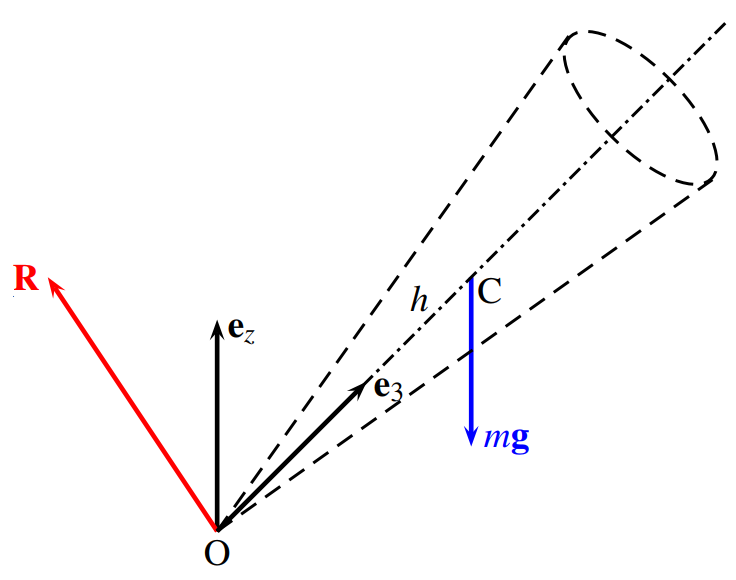
\includegraphics[width=7cm]{images/Toupie01.PNG} \end{center}
\end{tabular}





\item Projection sur $ \textbf{e}_z $ : $ \textbf{e}_z \cdot \dot{\textbf{H}}_O \implies \textbf{e}_z \cdot \textbf{H}_O = H_z = \text{const.} $, cette intégrale première exprimant la conservation de la composante verticale du moment cinétique. \\
En projetant sur \textbf{e}, il vient : $ \textbf{e}_z \cdot \dot{\textbf{H}}_O = 0 $. On utilise la dérivée relative par rapport aux axes liés au solide et l'équation devient :
\[ \textbf{e} \cdot \bigg[ \frac{\delta \textbf{H}_O}{\delta t} + \boldsymbol{\omega} \wedge \textbf{H}_O \bigg] = 0 \]
où : $\displaystyle \textbf{H}_O = \textbf{J}_O \cdot \boldsymbol{\omega} = A \boldsymbol{\omega} + (\Gamma - A) \; (\textbf{e} \cdot \boldsymbol{\omega}) \; \textbf{e} $ \\
$\displaystyle \implies \boldsymbol{\omega} \wedge \textbf{H}_O = (\Gamma - A) \; (\textbf{e} \cdot \boldsymbol{\omega}) \; (\boldsymbol{\omega} \wedge \textbf{e}) $ \\
$\displaystyle \implies \textbf{e} \cdot (\boldsymbol{\omega} \wedge \textbf{H}_O) = 0 $ \\
de sorte que, puisque \textbf{e} est constant dans les axes liés à la toupie, $\displaystyle \textbf{e} \cdot \frac{\delta \textbf{H}_O}{\delta t} = \frac{\delta}{\delta t} \big( \textbf{e} \cdot \textbf{H}_O \big) = 0 $. \\
Dès lors,
\[ \textbf{e} \cdot \textbf{H}_O = \Gamma \; \textbf{e} \cdot \boldsymbol{\omega} = \text{const.} \]
Cette intégrale première exprime la conservation du \emph{spin} : $ n = \textbf{e} \cdot \boldsymbol{\omega} $.


\end{enumerate} \end{siderules}










\section{Q1 Août 2016}





On considère une toupie présentant une symétrie de révolution d’axe \textbf{e} en mouvement autour de son sommet O fixe.
\begin{enumerate}

\item Définissez les angles d’Euler permettant de repérer l’orientation de la toupie dans l’espace et exprimez le vecteur de Poisson de la toupie en fonction de ceux-ci.

\item Exprimez et justifiez la forme particulière prise par le tenseur d’inertie de la toupie en O en raison de sa géométrie.

\item Établissez l’expression de l’énergie cinétique absolue de la toupie en fonction des angles d’Euler.

\end{enumerate}





\begin{siderules} \begin{enumerate}


\item Soit \textbf{e} l’axe de symétrie de révolution de la toupie et les vecteurs $ \textbf{e}_x $, $ \textbf{e}_y $ et $ \textbf{e}_z $ formant un repère d’orientation fixe. L’orientation de la toupie dans l’espace peut alors être décrite par la donnée des angles d’Euler suivants :

\begin{tabular}{M{7cm}M{7.5cm}}
\begin{enumerate}
    \item l’angle de nutation $ \theta $ mesure l’inclinaison de l’axe de référence \textbf{e} par rapport à la verticale $ \textbf{e}_z $ ;
    \item l’angle de précession $ \upvarphi $ mesure l’angle entre le plan formé par \textbf{e} et $ \textbf{e}_z $ et le plan formé par $ \textbf{e}_x $ et $ \textbf{e}_z $ ;
    \item l’angle de rotation propre $ \Uppsi $ mesure la rotation de la toupie autour de l’axe \textbf{e}. Le vecteur de Poisson peut être exprimé en fonction des angles d’Euler sous la forme :
    \[ \begin{aligned}
    \boldsymbol{\omega} &= \dot{\upvarphi} \; \textbf{e}_z + \dot{\Uppsi} \; \textbf{e} + \dot{\theta} \frac{\textbf{e}_z \wedge \textbf{e}}{\| \textbf{e}_z \wedge \textbf{e} \|} \\
    &= \dot{\upvarphi} \; \textbf{e}_z + \dot{\Uppsi} \; \textbf{e} + \frac{\dot{\theta}}{\sin \theta} (\textbf{e}_z \wedge \textbf{e})
    \end{aligned} \]
\end{enumerate}
&
\begin{center} 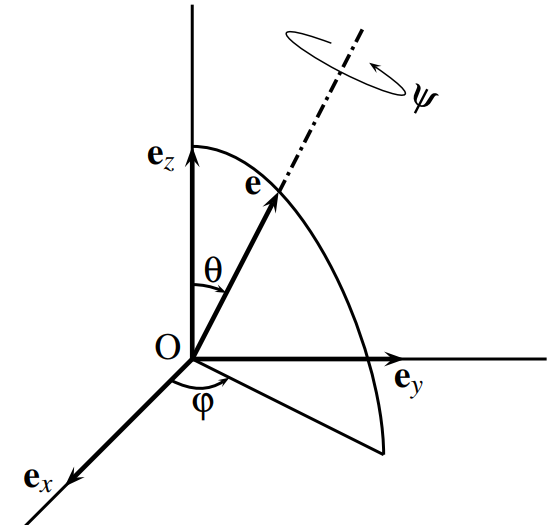
\includegraphics[width=7cm]{images/AnglesEuler.PNG} \end{center}
\end{tabular}





\item Voir le premier point de la Q1 de janvier 2017.





\item La toupie étant en rotation autour de son sommet O fixe, son énergie cinétique peut être exprimée sous la forme :
\[ \begin{aligned}
T_O &= \frac{1}{2} \boldsymbol{\omega} \cdot \textbf{J}_C \cdot \boldsymbol{\omega} = \frac{1}{2} \boldsymbol{\omega} \cdot \big[ A \; \textbf{I} + (\Gamma - A) \; \textbf{e} \textbf{e} \big] \cdot \boldsymbol{\omega} \\
&= \frac{A}{2} \omega^2 + \frac{1}{2} (\Gamma - A) \; (\boldsymbol{\omega} \cdot \textbf{e})^2 \\
&= \frac{A}{2} \big( \dot{\upvarphi}^2 + \dot{\Uppsi}^2 + \dot{\theta}^2 + \dot{\Uppsi} \dot{\upvarphi} \cos \theta \big) + \frac{1}{2} (\Gamma - A) \; (\dot{\Uppsi} + \dot{\upvarphi} \cos \theta)^2
\end{aligned} \]


\end{enumerate} \end{siderules}










\section{Q1 Janvier 2016}





\begin{enumerate}

\item Définissez les angles d’Euler permettant de repérer la position d’un gyroscope dans l’espace et exprimez le vecteur de Poisson du gyroscope en fonction de ceux-ci.

\item Quand dit-on qu’un gyroscope présente un mouvement de précession uniforme ?

\item Établissez l’expression du couple extérieur à appliquer à un gyroscope pour produire un mouvement de précession uniforme autour de son centre d’inertie.

\end{enumerate}





\begin{siderules} \begin{enumerate}


\item Voir le premier point de la Q1 d'août 2016.





\item On dit d’un gyroscope qu’il présente un mouvement de précession uniforme lorsque son axe de symétrie conserve une inclinaison constante par rapport à une direction fixe et tourne à vitesse angulaire constante autour de celle-ci. Dans ce mouvement, on a :
\[ \theta = \text{constante,} \qquad \dot{\upvarphi} = \text{constante,} \qquad \dot{\Uppsi} = \text{constante} \]





\item Lorsqu'on a un mouvement de précession uniforme, on a : $\displaystyle \boldsymbol{\omega} = \dot{\upvarphi} \; \textbf{e}_z + \dot{\Uppsi} \; \textbf{e} $, où $ \dot{\upvarphi} $ et $ \dot{\Uppsi} $ sont constantes. \\
Le gyroscope possède un tenseur central d'inertie de la forme : $\displaystyle \textbf{J}_C = A \; \textbf{I} + (\Gamma - A) \; \textbf{e} \textbf{e} $, où $ \Gamma $ et \emph{A} sont, respectivement, les moments principaux d’inertie pour la rotation autour de \textbf{e} et autour de tout axe perpendiculaire à \textbf{e}. \\
On calcule dès lors, 
\[ \textbf{H}_C = \textbf{J}_C \cdot \boldsymbol{\omega} = A \; \boldsymbol{\omega} + (\Gamma - A) \; (\dot{\Uppsi} + \dot{\upvarphi} \cos \theta) \; \textbf{e} \]
\[ \begin{aligned}
\dot{\textbf{H}}_C &= A \; \dot{\boldsymbol{\omega}} + (\Gamma - A) \; (\dot{\Uppsi} + \dot{\upvarphi} \cos \theta) \; \dot{\textbf{e}} \\
&= \dot{\upvarphi} \; \big[ \Gamma \dot{\Uppsi} + (\Gamma - A) \; \dot{\upvarphi} \cos \theta \big] \; \textbf{e}_z \wedge \textbf{e}
\end{aligned} \]
Appliquant le théorème du moment cinétique en \emph{C}, on en déduit que, pour provoquer une précession uniforme, il convient d’appliquer un couple extérieur de moment : 
\[ \textbf{M}_C = \dot{\upvarphi} \; \big[ \Gamma \dot{\upvarphi} + (\Gamma - A) \; \dot{\upvarphi} \cos \theta \big] \; \textbf{e}_z \wedge \textbf{e} \]
à la fois perpendiculaire à l’axe de symétrie du gyroscope et à l’axe autour duquel il précesse.


\end{enumerate} \end{siderules}










\section{Q1 Août 2015}





\begin{enumerate}

\item Établissez l’expression de l’énergie cinétique $ T_C $ d’un solide indéformable en fonction de son vecteur de Poisson si $ T_C $ est rapporté à un système d’axes centrés au centre d’inertie \emph{C} et constamment parallèles à des axes inertiaux. \\
Par rapport à quel(s) autre(s) point(s) une relation semblable existe-t-elle entre l’énergie cinétique et le vecteur de Poisson d’un solide ?

\item Déterminez, en justifiant, dans quel cas le mouvement d’un point matériel de 'masse variable' soumis à une force \textbf{F} peut être décrit par l’équation : $\displaystyle \frac{d}{d t} \big( m \; \dot{\textbf{s}} \big) = \textbf{F} $.

\item Définissez brièvement mais aussi complètement que possible les termes suivants : 
\begin{enumerate}
    \item Force conservative.
    \item Orbite géostationnaire.
    \item Toupie forte.
\end{enumerate}

\end{enumerate}





\begin{siderules} \begin{enumerate}


\item L’énergie cinétique d’un solide rapportée à un système d’axes centrés au centre d’inertie et constamment parallèles à des axes inertiaux est donnée par : $\displaystyle T_C = \frac{1}{2} \int \| \textbf{v}_r \|^2 \; d m $, où $ \textbf{v}_r $ désigne le vecteur vitesse par rapport au repère considéré. \\
On sait aussi que : 
\begin{equation}\tag{1}
\textbf{v}_r = \frac{\delta \textbf{r}}{\delta t} + \boldsymbol{\omega} \wedge \textbf{r} = \boldsymbol{\omega} \wedge \textbf{r}
\end{equation} puisque la position relative d’un point quelconque du solide est constante dans les axes liés au solide. Et on a donc : 
\[ \begin{aligned}
T_C &= \frac{1}{2} \int (\boldsymbol{\omega} \wedge \textbf{r}) \cdot (\boldsymbol{\omega} \wedge \textbf{r}) \; d m = \frac{1}{2} \int \boldsymbol{\omega} \cdot \big[ \textbf{r} \wedge (\boldsymbol{\omega} \wedge \textbf{r}) \big] \; d m = \frac{1}{2} \int \boldsymbol{\omega} \cdot \big[ (\textbf{r} \cdot \textbf{r}) \; \boldsymbol{\omega} - (\textbf{r} \cdot \boldsymbol{\omega}) \; \textbf{r}) \big] \; d m \\
&= \frac{1}{2} \int \|\textbf{r}\|^2 \|\boldsymbol{\omega}\|^2 - (\textbf{r} \cdot \boldsymbol{\omega})^2 \; d m
\end{aligned} \]
Avec le tenseur d'inertie en \emph{C} \Big($\displaystyle J_C = \int \|\textbf{r}\|^2 \textbf{I} - \textbf{r} \textbf{r} \; d m $\Big), il vient : 
\[ T_C = \frac{1}{2} \boldsymbol{\omega} \cdot \textbf{J}_C \cdot \boldsymbol{\omega} \]

Un relation semblable, $\displaystyle T_B = \frac{1}{2} \boldsymbol{\omega} \cdot \textbf{J}_B \cdot \boldsymbol{\omega} $, peut être écrite par rapport à n’importe quel système d’axes par rapport auquel le champ des vitesses peut être décrit par (1), i.e. par rapport à tout système d’axes parallèles à des axes inertiaux et centrés en un point \emph{B} fixe par rapport au solide. Le mouvement du solide par rapport à un tel référentiel se réduit à un mouvement de rotation.





\item L’équation du mouvement d’un point matériel de masse variable soumis à une force \textbf{F} s’écrit :
\begin{equation}\tag{2}
m \frac{d \dot{\textbf{s}}}{d t} = \textbf{F} + \textbf{P} = \textbf{F} + \frac{d m}{d t} \textbf{w}
\end{equation}
puisque la poussée \textbf{P} est donnée par : $\displaystyle \textbf{P} = \frac{d m}{d t} \textbf{w} $, où \textbf{w} est la vitesse relative par rapport au système à masse variable des matières qui vont être absorbées ou qui ont été éjectées. \\
L’équation donnée : $\displaystyle \frac{d}{d t} \big( m \; \dot{\textbf{s}} \big) = \textbf{F} $, peut s’écrire : 
\begin{equation}\tag{3}
m \frac{d \dot{\textbf{s}}}{d t} = \textbf{F} - \frac{d m}{d t} \dot{\textbf{s}}
\end{equation}
Les expressions (2) et (3) ne sont équivalentes que si : $ \textbf{w} = − \dot{\textbf{s}} $, c’est-à-dire si les matières qui vont être absorbées ou qui ont été éjectées sont au repos absolu.





\item \begin{enumerate}

\item Une force F est dite conservative si elle dérive d’un potentiel, i.e. si elle peut s’exprimer sous la forme : 
\[ \textbf{F} = - \nabla V(\textbf{s}) \]
où \emph{V} est une fonction de la position uniquement. \\
Le travail d’une force conservative déplaçant sont point d’application entre deux points A et B ne dépend pas du chemin \emph{C} suivi pour aller de A à B, i.e.
\[ \int_C \textbf{F} \cdot d \textbf{s} = - \int_C \nabla V \cdot d \textbf{s} = V(\textbf{s}_A) - V(\textbf{s}_B) \]

\item L’orbite géostationnaire est l’orbite équatoriale pour laquelle la vitesse angulaire de rotation du satellite autour de la Terre est précisément égale à la vitesse de rotation de la Terre sur elle-même. Tous les satellites de communication sont placés en orbite géostationnaire afin de rester à l’aplomb de la zone qu’ils doivent desservir. \\
Le rayon de l’orbite géostationnaire GEO est donné par :
\[ R_{\text{GEO}} = \sqrt[3]{\frac{G M T^2}{4 \pi^2}} \]
où \emph{T} est égal à un jour sidéral, \emph{M} est la masse de la Terre et \emph{G} la constante de Cavendish. L’altitude d’une telle orbite est approximativement de 35 800 kilomètres.

\item La toupie forte est un solide de révolution dont la rotation rapide autour de son axe de symétrie de révolution assure l’équilibre stable dans la position verticale supérieure. La toupie reste verticale en dépit de la force de pesanteur qui tend à faire basculer son axe de rotation lors de toute perturbation de l’équilibre.

\end{enumerate}


\end{enumerate} \end{siderules}










\section{Q1 Janvier 2015}





\begin{enumerate}

\item Déterminez l’expression du moment cinétique $ \textbf{H}_C $ d’un solide indéformable en fonction de son vecteur de Poisson si $ \textbf{H}_C $ est rapportée à un système d’axes centrés au centre d’inertie \emph{C} et constamment parallèles à des axes inertiaux.
Par rapport à quels autres points une relation semblable existe-t-elle entre le moment cinétique et le vecteur de Poisson d’un solide ?

\item À partir de la définition d’une force conservative, montrez que la puissance développée par une telle force peut s’exprimer comme l’opposé de la dérivée temporelle du potentiel.

\item Définissez brièvement mais aussi complètement que possible les termes suivants.
\begin{enumerate}
    \item Précession gyroscopique/effet gyroscopique.
    \item Équations d’Euler.
    \item Centre de percussion.
\end{enumerate}

\end{enumerate}





\begin{siderules} \begin{enumerate}


\item Quasi la même chose que la partie 1. de la Q1 d'août 2015 - $ T_C $ remplacé par $ \textbf{H}_C $. \\
Le moment cinétique rapporté à un système d’axes centrés au centre d’inertie d’un solide et constamment parallèles à des axes inertiaux est donné par : 
\[ \textbf{H}_C = \int \textbf{r} \wedge \textbf{v}_r \; d m \]
où \textbf{r} et $ \textbf{v}_r $ désignent respectivement le vecteur position et la vitesse par rapport au repère considéré. \\
On sait aussi que : 
\begin{equation}\tag{1}
\textbf{v}_r = \frac{\delta \textbf{r}}{\delta t} + \boldsymbol{\omega} \wedge \textbf{r} = \boldsymbol{\omega} \wedge \textbf{r}
\end{equation} puisque la position relative d’un point quelconque du solide est constante dans les axes liés au solide. Et on a donc : 
\[ \textbf{H}_C = \int \textbf{r} \wedge (\boldsymbol{\omega} \wedge \textbf{r}) \; d m = \int \Big[ \boldsymbol{\omega} \|\textbf{r}\|^2 - \textbf{r} (\textbf{r} \cdot \boldsymbol{\omega}) \Big] \; d m \]
Avec le tenseur d'inertie en \emph{C} \Big($\displaystyle J_C = \int \|\textbf{r}\|^2 \textbf{I} - \textbf{r} \textbf{r} \; d m $\Big), il vient : 
\[ \textbf{H}_C = \textbf{J}_C \cdot \boldsymbol{\omega} \]
Un relation semblable, $\displaystyle \textbf{H}_B = \textbf{J}_B \cdot \boldsymbol{\omega} $, peut être écrite par rapport à n’importe quel système d’axes par rapport auquel le champ des vitesses peut être décrit par (1), i.e. par rapport à tout système d’axes parallèles à des axes inertiaux et centrés en un point \emph{B} fixe par rapport au solide. Le mouvement du solide par rapport à un tel référentiel se réduit à un mouvement de rotation.





\item Une force \textbf{F} est dite conservative si elle dérive d’un potentiel, i.e. si elle peut s’exprimer sous la forme : 
\[ \textbf{F} = − \nabla V(\textbf{s}) \]
où \emph{V} est une fonction de la position uniquement. \\
Adoptant un repère cartésien de vecteurs unitaires $ \textbf{e}_x, \textbf{e}_y, \textbf{e}_z $, la puissance développée par une telle force est donnée par : 
\[ \begin{aligned}
\mathpzc{P} = \textbf{F} \cdot \dot{\textbf{s}} &= - \Big( \frac{\partial V}{\partial x} \textbf{e}_x + \frac{\partial V}{\partial y} \textbf{e}_y + \frac{\partial V}{\partial z} \textbf{e}_z \Big) \cdot (\dot{x} \textbf{e}_x + \dot{y} \textbf{e}_y + \dot{z} \textbf{e}_z) \\
&= \bigg[ \frac{\partial V}{\partial x} \frac{d x}{d t} + \frac{\partial V}{\partial y} \frac{d y}{d t} + \frac{\partial V}{\partial z} \frac{d z}{d t} \bigg] \\
&= - \frac{d V}{d t}
\end{aligned} \]





\item \begin{enumerate}

\item La précession gyroscopique ou effet gyroscopique est le mouvement de précession que présente un solide de révolution en rotation rapide autour de son axe de symétrie lorsqu’il est sollicité par un couple extérieur \textbf{C} indépendant de la vitesse de rotation. Au lieu de basculer dans la direction du couple appliqué, le solide acquiert un mouvement de rotation qui tend à aligner son axe de symétrie avec la direction du couple appliqué. Au premier ordre, la vitesse de précession : $ \dot{\upvarphi} \textbf{e}_z $ est telle que : 
\[ \textbf{C} = \gamma \dot{\upvarphi} \; \textbf{e}_z \wedge \dot{\Uppsi} \; \textbf{e} \]
où $ \Gamma $ désigne le moment d’inertie du solide par rapport à son axe de symétrie de révolution, \textbf{e} est le vecteur unitaire porté par cet axe de symétrie et : $ \dot{\Uppsi} >> \dot{\upvarphi} $ est la vitesse de rotation autour de cet axe.

\item Les équations d’Euler sont les équations scalaires obtenues en projetant sur les axes principaux d’inertie d’un solide le théorème du moment cinétique rapporté à des axes centrés au centre d’inertie (ou en un point fixe du solide) et constamment parallèles à des axes inertiaux, i.e.
\[ \begin{cases}
J_1 \dot{\omega}_1 + (J_3 - J_2) \; \omega_2 \omega_3 = M_1 \\
J_2 \dot{\omega}_2 + (J_1 - J_3) \; \omega_1 \omega_3 = M_2 \\
J_3 \dot{\omega}_3 + (J_2 - J_1) \; \omega_2 \omega_1 = M_3
\end{cases} \]
où $ (\omega_1, \omega_2, \omega_3) $ et $ (M_1, M_2, M_3) $ désignent les composantes dans les axes principaux d’inertie du vecteur de Poisson et du moment des forces appliquées au solide et où $ J_1, J_2, J_3 $ sont les moments principaux d’inertie.

\item Le centre de percussion d’un solide est le point auquel on peut appliquer des forces extérieures arbitrairement grandes, comme les forces impulsionnelles appliquées lors d’une percussion, sans provoquer de réaction aux appuis. \\
En frappant une boule de billard de rayon \emph{R} en son centre de percussion, situé à une distance $ 2 R / 5 $ au-dessus du centre d’inertie, on communique à la boule une vitesse de translation et une vitesse de rotation compatibles avec le roulement sans glissement sans qu’aucune force de frottement ne doive être mise en oeuvre au point de contact avec le plan. \\
Dans le cas d’une raquette de tennis, le centre de percussion correspond au point du tamis où il convient de frapper la balle pour éviter de faire naître un force de réaction importante au niveau du poignet.

\end{enumerate}



\end{enumerate} \end{siderules}


